\documentclass[12pt]{article}
\usepackage{preamble}

\pagestyle{fancy}
\fancyhead[LO,LE]{Специальные разделы \\ высшей математики}
\fancyhead[RO,RE]{Лекции Далевской О. П.}

\renewcommand{\thesection}{}

\begin{document}

    \tableofcontents
    \clearpage

        % begin specsec_2024_02_09.tex

    \section{1. Евклидовы пространства}


    \section{1.1. Скалярное произведение}

    $L$ - линейное пространство $\quad \forall x, y \in L \quad \underset{x, y \to c \in \Real}{c = (x, y) - \text{ск. произв.}}$

    \hypertarget{scalarproductdefinition}{}

    \begin{enumerate}
        \item $(x, y) = (y, x)$
        \item $(\lambda x, y) = \lambda (x, y), \quad \lambda \in \Real$
        \item $(x + z, y) = (x, y) + (z, y)$
        \item $\forall x \in L\ (x, x) \geq 0$ и $(x, x) = 0 \Longrightarrow x = 0$
    \end{enumerate}

    Если векторы и коэффициенты комплексно-значные, то определения будут другими!

    \Def Скалярная функция $c = (x, y)$ со свойствами 1-4 называется скалярным произведением элементов $x$ и $y$

    \hypertarget{euclidspacedefinition}{}

    \Def Линейное пространство со скалярным произведением называется \underline{Евклидовым}

    \ExN{1} ЛП - пространство геометрических векторов

    $(\overrightarrow{a}, \overrightarrow{b}) =
    \begin{sqcases}
        |\overrightarrow{a}||\overrightarrow{b}|\cos\varphi, \quad \overrightarrow{a}, \overrightarrow{b} \neq 0 \\
        0, \quad \overrightarrow{a} = 0 \lor \overrightarrow{b} = 0
    \end{sqcases}$

    \ExN{2} ЛП $= C_{[a;b]}$

    $(f(x), g(x)) \stackrel{def}{=} \int^b_a f(x)g(x) dx$

    Очевидно, что 1-3 выполняются, проверим 4:

    $\int^b_a f^2(x) dx = 0 \stackrel{?}{\Longrightarrow} f(x) = 0$

    \ExN{3} ЛП - пространство числовых строк вида $x = (x_1, x_2, \dots, x_n)$

    $(x, y) = x_1 y_1 + \dots x_n y_n = \sum_{i=1}^n x_i y_i$ - сумма произведений компонент

    \section{1.2. Свойства евклидова пространства - $E$}

    \hypertarget{inequalityofCauchyBunyakovsky}{}

    \Th Неравенство Коши-Буняковского

    $(x, y)^2 \leq (x, x)(y, y)$

    $\Box$

    Нетрудно заметить, что:

    $\sphericalangle (\lambda x - y, \lambda x - y) = (\lambda x - y, \lambda x) - (\lambda x - y, y) =
    (\lambda x, \lambda x) - (y, \lambda x) - (\lambda x, y) + (y, y) = \lambda^2 (x, x) - 2\lambda (x, y) + (y, y) \stackrel{\text{пусть}}{=} 0$

    Решим относительно $\lambda$

    $D = 4(x, y)^2 - 4(x, x)(y, y)$

    $\frac{D}{4} = (x, y)^2 - (x, x)(y, y)$

    Так как $(\lambda x - y) \geq 0$ (4-ое свойство ск. произв.), то уравнение имеет $\leq 1$ корня, значит
    $\frac{D}{4} = (x, y)^2 - (x, x)(y, y) \leq 0$

    $\Box$

    \section{1.3. Норма}

    \hypertarget{normdefinition}{}

    ЛП $= L, \forall x \in L$ определена функция так, что выполняется $x \to n \in \Real, n = \|x\|$

    \begin{enumerate}
        \item $\|x\| \geq 0$ и $\|x\| = 0 \Longrightarrow x = 0$
        \item $\|\lambda x\| = |\lambda| \cdot \|x\| \quad \lambda \in \Real$
        \item $\|x + y\| \leq \|x\| + \|y\| \quad \forall x, y \in L$ - неравенство треугольника
    \end{enumerate}

    \hypertarget{normalizedeuclidspace}{}

    Евклидово пространство с нормой называется нормированным

    \Th $E^n$ является нормированным, если $\|x\| = \sqrt{(x, x)}$

    $\Box$

    Свойства 1-2 очевидны, докажем 3 свойство:

    $\|x + y\| = \sqrt{(x + y, x + y)} \leq \sqrt{(x, x)} + \sqrt{(y, y)} = \|x\| + \|y\|$

    $\sqrt{(x, x) + 2(x, y) + (y, y)} \leq \sqrt{(x, x)} + \sqrt{(y, y)}$

    $(x, x) + 2(x, y) + (y, y) \leq (x, x) + (y, y) + 2\sqrt{(x, x)(y, y)}$

    $(x, y) \leq \sqrt{(x, x)(y, y)}$

    $(x, y)^2 \leq (x, x)(y, y)$ - верно по неравенству Коши-Буняковского

    $\Box$

    Обобщим геометрические понятия ортогональности и косинуса угла на случай произвольных векторов

    \Def $x, y$ - ортогональны, если $(x, y) = 0$ и $x \neq 0$ и $y \neq 0 \quad x \perp y$

    \Def $\cos(\widehat{x, y}) = \frac{(x, y)}{\|x\|\cdot\|y\|}$ - косинус угла между векторами

    \Def $x, y \in E^n \quad x \perp y \quad z = x + y$ - гипотенуза

    \Th $x \perp y$, тогда $\|x + y\|^2 = \|x\|^2 + \|y\|^2$

    $\Box$

    $\|x + y\|^2 = (x + y, x + y) = (x, x)^2 + \underset{= 0, x \perp y}{\undergroup{2(x, y)}} + (y, y)^2 = (x, x)^2 + (y, y)^2$

    $\Box$

    \Def $B = \Set{e_i}_{i=1}^n$ - базис $L^n$

    На $L^n$ введены $(x, y)$ и $\|x\|$ (то есть $L^n \to E^n_{\|\cdot\|}$ - нормированное евклидово)

    \hypertarget{ortonormalizedbasis}{}

    $B$ называют ортонормированным базисом, если $(e_i, e_j) = \begin{cases}0, i \neq j \\ 1, i = j\end{cases}$

    \Nota Докажем, что всякая такая система из $n$ векторов линейно независима (то есть всякая нулевая комбинация тривиальная):

    $\sum_{i=1}^n \lambda_i e_i = 0 \stackrel{?}{\Longrightarrow} \forall \lambda_i = 0$

    $(e_k, \sum_{i=1}^n \lambda_i e_i) = \sum_{i=1}^n \lambda_i (e_k, e_i) \stackrel{k \neq i \Rightarrow (e_k, e_i) = 0}{=\joinrel=\joinrel=}
    \lambda_k \|e_k\|^2 = \lambda_k = 0 \quad \forall k$
    % end {i}

    % begin specsec_2024_02_16.tex

    \hypertarget{orthogonalbasisinspace}{}

    \Th Во всяком $E^n$ можно выделить ортонормированный базис

    $\Box$

    В $E^n_{\|\cdot\|} \ \exists B = \{\beta_1, \dots, \beta_n\}$ - базис

    ? Можно ли выделить $\mathcal{E} = \{e_1, \dots, e_n\}$ - ортонормированный базис?

    Метод мат. индукции:

    База: построим один ортогональный вектор для $\beta_1 = e_1^\prime$ (потом $e_1 = \frac{e_1^\prime}{\|e_1^\prime\|}$)

    Рассмотрим $e_2^\prime = \beta_1 - \lambda e^\prime_1$. Требуем $e_2^\prime \perp e_1^\prime$, то есть $(e_1^\prime, e_2^\prime) = 0$

    Отсюда найдем нужный $\lambda: (e_1^\prime, e_2^\prime) = (e_1^\prime, \beta_2 - \lambda e_1^\prime) = (e_1^\prime, \beta_2) - \lambda (e_1^\prime, e_1^\prime) = 0$

    Тогда $\lambda = \frac{(e_1^\prime, \beta_2)}{(e_1^\prime, e_1^\prime)}$

    Переход: Пусть построена система ортогональных векторов $\{e_1^\prime, e_2^\prime, \dots, e_k^\prime\}$

    Построим $k + 1$ систему:

    Рассмотрим $e_{k+1}^\prime = \beta_{k + 1} - \lambda_k e_k^\prime - \lambda_{k - 1}^\prime e_{k - 1}^\prime - \dots - \lambda_1 e_1^\prime \quad (*)$

    Требуем $e_{k+1}^\prime \perp e_i \quad \forall i \in [1;k]$

    $(e_{k+1}^\prime, e_k^\prime) = (\beta_{k + 1}, e_k^\prime) - \lambda_k (e_k^\prime, e_k^\prime) = 0$, так как $(e_i^\prime, e_j^\prime) = 0 \quad i \neq j$

    $\lambda_k = \frac{(\beta_{k + 1}, e_k^\prime)}{(e_k^\prime, e_k^\prime)}$

    Аналогично: $(e_{k+1}^\prime, e_{k - 1}^\prime) = (\beta_{k+1}, e_{k - 1}^\prime) - \lambda_{k - 1}(e_{k - 1}^\prime, e_{k-1}^\prime)$

    $\lambda_{k - 1} = \frac{(\beta_{k + 1}, e_{k - 1}^\prime)}{(e_{k - 1}^\prime, e_{k - 1}^\prime)}$

    $\Box$

    Изложенный метод называется методом ортогонализации базиса, при этом $(*)$ определяет ненулевой вектор, иначе получим нулевую тривиальную линейную комбинацию векторов $\beta_i$ ($e_i$ выражается через них), но это невозможно, так как вектора базисные.

    Полученную систему стоит нормировать

    \Ex Формула скалярного произведения в о/н базисе

    $E_{\|\cdot\|}, B = \{\beta_1, \dots, \beta_n\}$ - какой-либо базис

    Рассмотрим $x = x_1 \beta_1 + x_2 \beta_2 + \dots + x_n \beta_n$ и $y = y_1 \beta_1 + \dots + y_n \beta_n$

    Найдем $(x, y)$, как произведение компонент: $(x_1 \beta_1 + \dots + x_n \beta_n, y_1 \beta_1 + \dots + y_n \beta_n) = \sum_{i = 1}^n \sum_{j = 1}^n x_i y_j (\beta_i, \beta_j)$

    Обозначим $(\beta_i, \beta_j) = a_{ij} \in \Real$

    Таким образом, $(x, y) = \sum_i \sum_j a_{ij} x_i y_j$ - дальше назовем квадратичной формой

    Ранее (в аналитической геометрии) $(a, b) = \sum_{i = 1}^n a_i b_i$ - произведение координат векторов $\vec{a}, \vec{b}$ в ДПСК (с о/н базисом)

    Действительно: если $\beta_i = e_i$, $\beta_j = e_j$, $e_{ij} \in $ о/н базису

    $a_{ij} = \begin{sqcases}1, i = j \\ 0, i \neq j\end{sqcases}$

    Таким образом, $(x, y) = \sum_{i = 1}^n x_i, y_i$

    Причем $x = x_1 e_1 + \dots + x_n e_n \Longrightarrow x_i = (x, e_i)$

    \Ex Система функций, непрерывных на $[0, 2\pi]$

    $\Phi = \{1, \sin t, \cos t, \sin 2t, \dots, \sin nt, \cos nt\}$

    Система ортогональна (\Lab), но не нормированная (\Lab)

    $\Phi_{\|\cdot\|} = \{\frac{1}{\sqrt{2\pi}}, \frac{1}{\sqrt{\pi}}\sin t, \frac{1}{\sqrt{\pi}} \cos t, \dots\}$ - нормированная система

    Тогда функция, определенная и непрерывная на $[0, 2\pi]$ может быть разложена по базису $\Phi_{\|\cdot\|}$
    и ее координат (как вектора): $f_i = \int_0^{2\pi} f \cdot e_i dx$, где $e_i \in \Phi_{\|\cdot\|}$
    % end {i}

    % begin specsec_2024_03_01.tex

    \Nota Изоморфизм $E^n \rightarrow E^{\prime n}$ позволяет переносить свойства скалярного произведения
    из одного в другое пространство

    Ex: $\|x + y\| \leq \|x\| + \|y\|$ - арифметические векторы со скалярным произведением $(x, y) = \Sigma^n_{i=1} x_i y_i$

    $E^{\prime n} \in C_{[a;b]}$ со скалярным произведением $\displaystyle (f, g) = \int^b_a f * g dx$

    $\displaystyle \sqrt{\int^b_a (f * g)^2 dx} \leq \sqrt{\int^b_a f^2 dx} + \sqrt{\int^b_a g^2 dx}$

    \hypertarget{perpendicularproblem}{}

    \section{1.4. Задача о перпендикуляре}

    Постановка: Нужно опустить перпендикуляр из точки пространства $E^n$ на подпространство $G$

    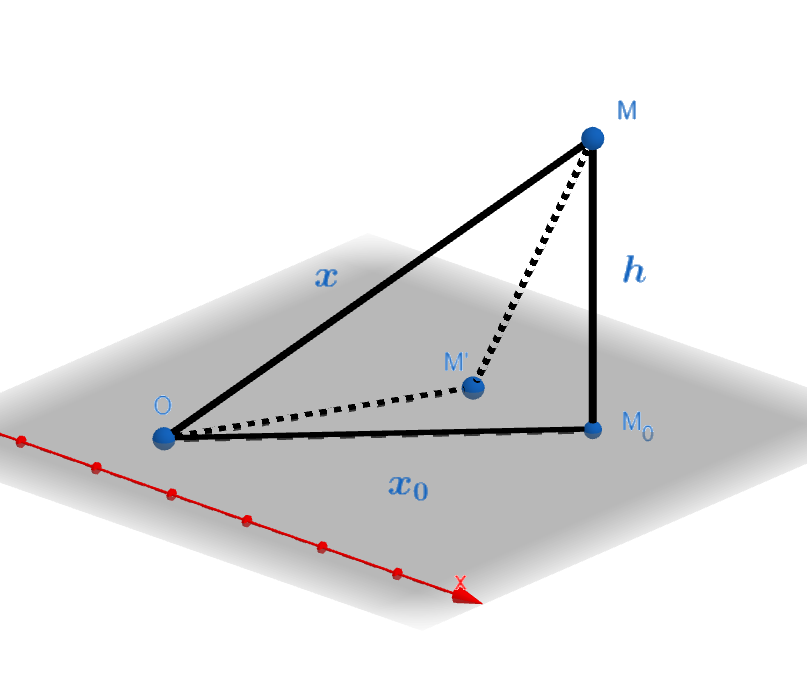
\includegraphics[height=90mm]{specsec/images/specsec_2024_03_01_1}

    Точка $M$ - конец вектора $x$ в пространстве $E^n$.
    Нужно найти $M_0$ (конец вектора $x_0$, проекции $x$ на $G$)

    \[x_0 + h = x\]

    где $h \perp G$. Правда ли что, длина перпендикулярного вектора $h$ - минимальная длина от точки $M$ до $G$?

    \Th $h \perp G, x_0 \in G, x = x_0 + h$. Тогда $\forall x^\prime \in G (x^\prime \neq x_0) \ \ \|x - x^\prime\| > \|x - x_0\|$

    $\Box \|x - x^\prime\| = \|x - x_0 + x_0 - x^\prime\| \stackrel{\text{по теореме Пифагора}}{=\joinrel=\joinrel=\joinrel=} \|x - x_0\| + \|x_0 - x^\prime\| = \|h\| + \|x_0 - x^\prime\| > \|x - x_0\|$

    \Nota $x_0$ называется ортогональной проекцией, возникает вопрос о ее вычислении (так находятся основания перпендикуляров)

    \vspace{5mm}

    \textit{Алгоритм:} $x_0 = \lambda_1 e_1 + \lambda_2 e2 + \dots + \lambda_k + e_k$, $\{e_i\}^k_{i=1}$ - базис $G$ (необязательно ортонормированный)

    Дан вектор $x$, пространство $G$, нужно найти $\lambda_i$

    $h = x - x_0$, $h \perp G \quad  (h, e_i) \stackrel{h \perp e_i \ \forall i}{=} 0$

    $(x - x_0, e_i) = (x, e_i) - (x_0, e_i) = 0$

    $(x, e_i) = (x_0, e_i)$

    Тогда $\forall i \quad (x_0, e_i) = (\lambda_1 e_1 + \dots + \lambda_k e_k, e_i) = \lambda_1 (e_1, e_i) + \dots + \lambda_k (e_k, e_i)$ - $(e_k, e_i)$ - числа, а $\lambda_i$ - неизвестные

    Получили СЛАУ:

    $\begin{array}{|cccc|}
    (e_1, e_1) & (e_1, e_2) & \ldots & (e_1, e_k)\\
    \ldots & \ldots & \ldots & \ldots\\
    (e_k, e_1) & (e_k, e_2) & \ldots & (e_k, e_k)\\
    \end{array} \times \begin{array}{|c|}
    \lambda_1\\
    \ldots\\
    \lambda_k \\
    \end{array} = \Gamma \times \begin{array}{|c|}
    \lambda_1\\
    \ldots\\
    \lambda_k \\
    \end{array} = \begin{array}{|c|}
    (x,e_1)\\
    \ldots\\
    (x,e_k) \\
    \end{array}$

    \Nota В матрице $\Gamma$ нет нулевых строк, так как $e_i$ - бизисная и по крайней мере $e_i^2 \neq 0$

    Таким образом по теореме Крамера $\exists! (\lambda_1, \dots, \lambda_k)$

    \hypertarget{grammatrix}{}

    \Def Матрицу $\Gamma = {(e_i, e_j)}_{i, j = 1\dots k}$ называют матрицей Грама

    $\Gamma = I = \begin{array}{|ccc|}
    1 & 0 & \ldots\\
    0 & 1 & \ldots\\
    \ldots & \ldots & 1\\
    \end{array}$, если базис ортонормированный

    Далее, $I$ - единичная матрица Грама

    \Nota Тогда $I \times \begin{array}{|c|}
    \lambda_1\\
    \ldots\\
    \lambda_k \\
    \end{array} = \begin{array}{|c|}
    \lambda_1\\
    \ldots\\
    \lambda_k \\
    \end{array} = \begin{array}{|c|}
    (x,e_1)\\
    \ldots\\
    (x,e_k) \\
    \end{array}$

    \vspace{5mm}

    \textbf{Приложения задачи о перпендикуляре}

    1) Метод наименьших квадратов

    В качестве простейшей модели зависимости $y = y(x)$ берем линейную функцию $y = \lambda x$

    Ищем минимально отстоящую прямую от данных $(x_i, y_i)$, то есть ищем $\lambda$

    Определим расстояние (в этом методе) как $\sigma^2 = \Sigma^n_{i=1} (y_i - y_{0i})^2 = \Sigma^n_{i=1} (y_i - \lambda x_i)^2$ - минимизируем

    Таким образом, ищем $y_0$ (ортог. проекция) такое, что $(y - y_0)^2 = \sigma^2$ - минимальное

    Если $y_0 = \lambda_1 x_1 + \dots + \lambda_k x_k$, где $x_i$ - набор измерений для $i$-ой точки

    Рассмотрим $y_0$ как разложение по базису $\{x_i\}$

    \vspace{5mm}

    2) Многочлен Фурье

    $P(t) = \frac{a_0}{2} + a_1 \cos t + b_1 \sin t + \dots a_n \cos nt + b_n \sin nt$ - линейная комбинация

    Функции ${1, \cos t, \sin t, \dots, \cos nt, \sin nt}$ - ортогональны

    Задача в том, чтобы для функции $f(t)$, определенной на отрезке $[0;2\pi]$ найти минимально отстоящий многочлен $P(t)$ при том,
    что расстояние определяется как $\displaystyle \sigma^2 = \int_0^{2\pi} (f(t) - P(t))^2 dt$

    Нужно найти $a_i$ и $b_i$ - обычные скалярные произведения $\displaystyle a_i = k \int_0^{2\pi} f(t) \cos(it) dt$, $\displaystyle b_i = m \int_0^{2\pi} f(t) \sin(it) dt$ ($k, m$ - нормирующие множители)

    \clearpage

    \section{2. Линейный оператор (линейное отображение, линейный функционал, линейное преображение)}

    \hypertarget{linearoperatordefinition}{}

    \section{2.1. Определение}

    \textit{Линейный оператор} - это отображение $V^n \stackrel{\mathcal{A}}{\Longrightarrow} W^m$

    ($V^n, W^m$ - линейные пространства размерности $n \neq m$ в общем случае),

    которое $\forall x \in V^n$ сопоставляет один какой-либо $y \in W^m$ и

    $\mathcal{A} (\lambda x_1 + \mu x_2) = \lambda \mathcal{A} x_1 + \mu \mathcal{A} x_2 = \lambda y_1 + \mu y_2$

    \Nota Заметим, что если 0 представим как $0 * x$, где $x \neq 0$, то

    $\mathcal{A}(0) = \mathcal{A}(0 * x) = 0 * \mathcal{A}x \stackrel{0 * y}{=} 0$

    \Nota Если $V = W$, то $\mathcal{A}$ называют линейным преобразованием, но далее будем рассматривать в основном операторы $\mathcal{A}: \ \ V \rightarrow V$, $\mathcal{A}: \ \ V^n \rightarrow W^n$



    \ExN{1} $V = \Real^2$ - пространство направленных отрезков

    $\mathcal{A}: V \leftarrow V$

    $\mathcal{A}x = y = \lambda y_1 + \mu y_2$ для таких $\mathcal{A}$ как сдвиг, поворот, гомотетия, симметрия

    \ExN{2} $V^n = W^m$, где $m < n$

    $\mathcal{A}$ - оператор проектирования (убедиться, что он линейный)

    \ExN{3} $V^n$ - пространство числовых строк длины $n$

    $\mathcal{A}: V^n \leftarrow V^n$

    $x = (x_1, \dots, x_n), y = (y_1, \dots, y_n)$

    $\mathcal{A}x = y : \begin{array}{|ccc|}
    a_{11} & \ldots & a_{1n}\\
    \vdots & \ddots & \vdots\\
    a_{n1} & \ldots & a_{nn}\\
    \end{array}x = y$


    \section{2.2. Действия с операторами}

    \Def $\mathcal{A}\mathcal{B}: V \rightarrow W$

    \begin{enumerate}
        \item $(\mathcal{A} + \mathcal{B})x \stackrel{def}{=} \mathcal{A}x + \mathcal{B}x$ - определение суммы $\mathcal{A} + \mathcal{B} = \mathcal{C}$
        \item $(\lambda\mathcal{A})x \stackrel{def}{=} \lambda(\mathcal{A}x)$ - $\lambda\mathcal{A} = \mathcal{D}$
    \end{enumerate}

    \Nota Сформируем линейное пространство из операторов $\mathcal{A}: V \rightarrow W$

    \begin{enumerate}
        \item Ассоциативность сложения (очевидно)
        \item Коммутативность (очевидно)
        \item Нейтральный элемент $\mathcal{O}x = 0$
        \item Противоположный: $-\mathcal{A} = (-1) * A$
        \item \dots \textit{LAB}
    \end{enumerate}

    \textit{Def:} $\mathcal{I}$ - тождественный - $\forall x \in V \ \ \mathcal{I}x = x$
    % end {i}

    % begin specsec_2024_03_15.tex

    \Def Произведение операторов (композиция)

    $\mathcal{A}\mathcal{B}$ - произведение, $\mathcal{A} : V \rightarrow W; \ \mathcal{B} : U \rightarrow V$

    $(\mathcal{A}\mathcal{B}) x = \mathcal{A}(\mathcal{B}x); \quad x \in U$

    \hypertarget{linearoperatorproperties}{}

    Свойства: \underline{Lab} доказать

    1* $\lambda (\mathcal{A}\mathcal{B}) = (\lambda \mathcal{A})\mathcal{B}$

    2* $(\mathcal{A} + \mathcal{B}) \mathcal{C} = \mathcal{A}\mathcal{C} + \mathcal{B}\mathcal{C}$

    3* $\mathcal{A} (\mathcal{B} + \mathcal{C}) = \mathcal{A}\mathcal{B} + \mathcal{A}\mathcal{C}$

    4* $\mathcal{A} (\mathcal{B}\mathcal{C}) = (\mathcal{A}\mathcal{B}) \mathcal{C}$


    \Nota Можно обобщить 4* на $n$ равных $\mathcal{A}$

    \Def $\mathcal{A}^n = \mathcal{A} \cdot \mathcal{A} \dots \mathcal{A}$ - $n$ раз, степень оператора

    Свойства: $\mathcal{A}^{m + n} = \mathcal{A}^n \cdot \mathcal{A}^m$

    \section{2.3. Обратимость оператора}

    \hypertarget{onetoonelinearoperator}{}

    Def: $\mathcal{A} : V \rightarrow W$ так, что $\mathcal{A}V = W$ и $\forall x_1 \neq x_2 (x_1, x_2 \in V) \quad
    \begin{cases}y_1 = \mathcal{A}x_1 \\ y_2 = \mathcal{A}x_2\end{cases} \Longrightarrow y_1 \neq y_2$

    Тогда $\mathcal{A}$ называется взаимно-однозначно действующим

    Nota: Проще сказать \enquote{линейный изоморфизм}

    \Th $\Set{x_i}$ - линейно независима $\stackrel{\mathcal{A}x = y}{\longrightarrow} \Set{y_i}$ - линейно независима

    В обратную сторону, если $\mathcal{A}$ - взаимно-однозначен

    $\Box \sqsupset \mathcal{A} : V \rightarrow W$ и $\texttt{0}_V, \texttt{0}_W$ - нули $V$ и $W$ соответственно
    \begin{enumerate}
        \item $\mathcal{A}(\texttt{0}_V) = \mathcal{A}(\sum^k_{i=1} 0 \cdot e_i) = \sum^k_{i=1} 0 \cdot \mathcal{A}e_i = \texttt{0}_W$

        \item Докажем, что если ${x_i} \subset V$ - лин. нез., то ${y_i} \subset W$ - лин. нез.

        Составим $\sum^m_{j=1} \lambda_j y_j = \texttt{0}_W$ (От противного) $\sqsupset \Set{y_i}$ - лин. зав., тогда $\exists \lambda_k \neq 0$

        При этом $\forall j \ \ y_j = \mathcal{A}x_j$ (т. к. $\mathcal{A}$ - вз.-однозн., то $n^\prime = m^\prime$: кол-во $x_i$ и $y_i$ равно)

        $\sum^{m^\prime}_{j=1} \lambda_j \mathcal{A}x_j \stackrel{\text{линейность}}{=} \mathcal{A} (\sum^{m^\prime}_{j=1} \lambda_j x_j) = \texttt{0}_W$

        Так как $\mathcal{A}\texttt{0}_V = \texttt{0}_W$, то $\texttt{0}_W$ - образ $x = \texttt{0}_V$, но так как $\mathcal{A}$ - вз.-однозн., то
        $\nexists x^\prime \neq x \ | \ \mathcal{A}(x^\prime) = \texttt{0}_W$

        Значит $\sum^{m^\prime}_{j=1} \lambda_j x_j = \texttt{0}_V$, но $\exists \lambda_k \neq 0 \Longrightarrow \Set{x_j}$ - лин. зав. - \underline{противоречие}

        \item $\sqsupset$ теперь $\Set{y_i}$ - л. нез., а $\Set{x_i}$ (по предположению от противного) - лин. зав.

        $\sum^{n^\prime}_{i = 1} \lambda_i x_i \stackrel{\exists \lambda_k \neq 0}{=} \texttt{0}_V \quad \Big| \mathcal{A}$

        $\sum^{n^\prime}_{i = 1} \lambda_i \mathcal{A}x_i = \texttt{0}_W$

        При этом $\exists \lambda_k \neq 0 \Longrightarrow \Set{y_i}$ - лин. зав. - \underline{противоречие}

    \end{enumerate}

    Следствие: $\dim V = \dim W \Longleftarrow \mathcal{A}$ - лин. изоморфизм

    \hypertarget{reverselinearoperator}{}

    Def: $\mathcal{B} : W \rightarrow V$ называется обратным оператором для $\mathcal{A} : V \rightarrow W$

    если $\mathcal{B}\mathcal{A} = \mathcal{A}\mathcal{B} = \mathcal{I}$ (обозначается $\mathcal{B} = \mathcal{A}^{-1}$)

    Следствие: $\mathcal{A}\mathcal{A}^{-1} x = x$

    \Th $\mathcal{A}x = \texttt{0}$ и $\exists \mathcal{A}^{-1}$, тогда $x = \texttt{0}$

    $\Box \mathcal{A}^{-1}\mathcal{A} x = \mathcal{A}^{-1}(\mathcal{A} x) = \mathcal{A}^{-1} \texttt{0}_W = \texttt{0}_V \Longrightarrow x = \texttt{0}$

    \Th Необходимые и Достаточные условия существования $\mathcal{A}^{-1}$

    $\exists \mathcal{A}^{-1} \Longleftrightarrow \mathcal{A}$ - вз.-однозн.

    $\Box \Longrightarrow \exists \mathcal{A}^{-1}$, но $\sqsupset \mathcal{A}$ - не вз.-однозн., то есть
    $\exists x_1, x_2 \in V (x_1 \neq x_2) \ | \ \mathcal{A}x_1 = \mathcal{A}x_2 \Longleftrightarrow \mathcal{A}x_1 - \mathcal{A}x_2 = \texttt{0} \Longleftrightarrow
    \mathcal{A}(x_1 - x_2) = \texttt{0}_W \stackrel{\exists \mathcal{A}^{-1}}{\Longrightarrow} x = \texttt{0}_V \Longleftrightarrow x_1 = x_2$ - противоречие

    $\Longleftarrow$ Так как $\mathcal{A}$ - изоморфизм (не учитывая линейность), то $\exists \mathcal{A}^\prime$ - обратное отображение (не обязат. линейное)

    Докажем, что $\mathcal{A}^\prime : W \rightarrow V$ - линейный оператор

    ? $\mathcal{A}^\prime (\sum \lambda_i y_i) = \sum \lambda_i \mathcal{A}^\prime y_i = \sum \lambda_i x_i$

    $\mathcal{A}$ - вз.-однозн. $\Longleftrightarrow \forall x_i \longleftrightarrow y_i \quad \Big| \cdot \lambda_i, \sum$

    $\mathcal{A}(\sum \lambda_i x_i) = \mathcal{A} x = y = \sum \lambda_i y_i \quad$ и $y$ имеет только один прообраз $x$

    Применим $\mathcal{A}^\prime$ к $y = \sum \lambda_i y_i \quad \mathcal{A}^\prime y = x = \sum \lambda_i x_i$ - единственный прообраз $y$

    Таким образом, $\mathcal{A}^\prime$ переводит лин. комбинацию в такую же лин. комбинацию прообразов, то есть $\mathcal{A}^\prime$ - линейный: $\mathcal{A}^\prime = \mathcal{A}^{-1}$

    \section{2.4. Матрица ЛО}

    $\mathcal{A} : V^n \rightarrow W^m$

    Возьмем вектор $x \in V^n$ и разложим по какому-либо базису $\Set{e_j}^n_{j=1}$

    $\mathcal{A}x = \mathcal{A} (\sum^n_{j=1} c_j e_j) = \sum^n_{j=1} c_j \mathcal{A}e_j$

    $\mathcal{A} e_j \stackrel{\text{образ базисного вектора}}{=} y_j \stackrel{\Set{f_i} - \text{ базис } W^m}{=} \sum^m_{i=1} a_{ij}f_i$

    $\mathcal{A}x = \sum^n_{j=1} c_j \mathcal{A}e_j = \sum^n_{j=1} c_j \sum^m_{i=1} a_{ij}f_i = \sum^n_{j=1} \sum^m_{i=1} c_j a_{ij} f_i = \sum^m_{i=1} \sum^n_{j=1} c_j a_{ij} f_i$

    Иллюстрация:

    $\begin{pmatrix}
         a_{11} & \dots & a_{1n} \\
         \vdots & \ddots & \vdots \\
         a_{m1} & \dots & a_{mn} \\
    \end{pmatrix} \begin{pmatrix}
         c_{1} \\
         \vdots \\
         c_{n} \\
    \end{pmatrix} = \begin{pmatrix}
         b_{1} \\
         \vdots \\
         b_{m} \\
    \end{pmatrix}$

    \hypertarget{operatorsmatrix}{}

    Def: Матрица $A = {a_{ij}}_{i=1..m, j=1..n}$ называется матрицей оператора $\mathcal{A} : V^n \rightarrow W^m$ в базисе $\Set{e_j}^n_{j=1}$ пространства $V^n$

    Вопросы:

    1) $\forall ? \mathcal{A} \ \exists A$

    2) $\forall ? A \ \exists \mathcal{A}$

    3) если $\exists A$ для $\mathcal{A}$, то единственная?

    4) если $\exists \mathcal{A}$ для $A$, то единственная?

    Ответы:

    1) При выбранном базисе $\Set{e_j} \ \forall \mathcal{A} \ \exists A$ (алгоритм выше)

    3) такая $A$ единственная $\Longrightarrow$ в разных базисах матрицы ЛО $\mathcal{A} \quad A_e \neq A_{e^\prime}$

    2) $\forall A_{m\times n}$ можно взять пару ЛП $V^n, W^m$ и определить $\mathcal{A} : V^n \rightarrow W_n$ по правилу $\mathcal{A}e_V = e_W^\prime$

    4) \Lab

    Nota: Далее будем решать две задачи

    1) преобразование координат как действие оператора

    2) поиск наиболее простой матрицы в некотором базисе

    \section{2.5. Ядро и образ оператора}

    \hypertarget{kernalandimageofoperator}{}

    \Def Ядро оператора - $Ker \mathcal{A} \stackrel{def}{=} \Set{x \in V \ | \ \mathcal{A}x = \texttt{0}_W}$

    \Def Образ оператора - $Im \mathcal{A} \stackrel{def}{=} \Set{y \in W \ | \ \mathcal{A}x = y}$

    \Nota $Ker \mathcal{A}$ и $Im \mathcal{A}$ - подпространства
    % end {i}

    % begin specsec_2024_03_22.tex

    \Nota $Ker\ \mathcal{A}$ и $Im\ \mathcal{A}$ - подпространства $V$ ($\mathcal{A} : V \rightarrow V$)

    Вообще-то $Ker\ \mathcal{A} \subset V, Im\ \mathcal{A} \subset W \ (\mathcal{A} : V \rightarrow W)$

    $\dim W \leq \dim V$, тогда можно считать, что $W \subset V^\prime$ и
    рассмотрим $\mathcal{A} : V \rightarrow V^\prime$ (где $V^\prime$ изоморфен $V$)

    $Ker \mathcal{A}$ - подпространство, то есть $Ker \mathcal{A} \subset V$ и
    $\sum c_i x_i \subset \mathcal{A}$, если $\forall x_i \in Ker \mathcal{A}$

    $\mathcal{A} (\sum c_i x_i) = \sum c_i \mathcal{A} x_i \stackrel{x_i \in \mathcal{A}}{=} \sum c_i \texttt{0} = \texttt{0}$

    Следствие: $Ker \mathcal{A} = \texttt{0} \Longrightarrow \mathcal{A}$ - вз.-однозн.

    $\Box$ От противного:

    $\sqsupset \mathcal{A}$ - не вз.-однозн., то есть $\exists x_1, x_2 \in V (x_1 \neq x_2) | \mathcal{A}x_1 = \mathcal{A}x_2 \Longleftrightarrow \mathcal{A} (x_1 - x_2) = \texttt{0} \Longrightarrow x_1 - x_2 \in Ker \mathcal{A}$ - противоречие

    \Nota Обратное также верно:

    $\mathcal{A}$ - вз.-однозн. $\Longleftrightarrow y_1 = y_2 \Longrightarrow x_1 = x_2$, так как $\mathcal{A}(x_1 - x_2) = \texttt{0} \Longrightarrow x_1 - x_2 = 0$

    Тогда $\texttt{0}$ является образом только $\texttt{0}$-вектора $\Longrightarrow Ker \mathcal{A} = \texttt{0}$

    \Nota Также очевидно, что

    $Ker \mathcal{A} = 0 \Longleftrightarrow Im \mathcal{A} = V$

    $Ker \mathcal{A} = V \Longrightarrow Im \mathcal{A} = \texttt{0}$ и $\mathcal{A} = 0$

    \hypertarget{theoremaboutdimensions}{}

    \Th $\mathcal{A} : V \rightarrow V$, тогда $\dim Ker \mathcal{A} + \dim Im \mathcal{A} = \dim V$

    $\Box$ Так как $Ker \mathcal{A}$ - подпространство $V$, то можно построить дополнение до прямой суммы (взяв базисные векторы ядра, дополнить их набор до базиса $V$: $e^k_1, \dots e^k_m, e^k_{m+1}, \dots e^k_n$)

    Обозначим дополнение $W$, тогда $Ker \mathcal{A} \xor W = V \Longrightarrow \dim Ker \mathcal{A} + \dim W = \dim V$

    Докажем, что $W$ и $Im \mathcal{A}$ - изоморфны

    $\mathcal{A} : W \rightarrow Im \mathcal{A}$

    $\mathcal{A} : Ker \mathcal{A} \rightarrow \texttt{0}$

    Докажем, что $\mathcal{A}$ действует из $W$ в $Im \mathcal{A}$ взаимно-однозначно

    $\sqsupset \mathcal{A}$ невз.-однозн., тогда $\exists x_1, x_2 \in W (x_1 \neq x_2) | \mathcal{A}x_1 = \mathcal{A}x_2 \in Im \mathcal{A}$

    $\mathcal{A}(x_1 - x_2) = \texttt{0} \Longrightarrow x_1 - x_2 \stackrel{\text{обозн.}}{=} x \in Ker \mathcal{A}$, но $x \neq 0$, так как $x_1 \neq x_2$

    Но для прямой суммы $W \union Ker \mathcal{A} = \texttt{0}, x \ni W \union Ker \mathcal{A} \Longrightarrow$ предположение неверно

    $\Longrightarrow \mathcal{A}$ - лин. вз.-однозн. $\Longrightarrow \dim W = \dim Im \mathcal{A}$

    $V = W_1 \xor W_2$ найдется ЛО $\mathcal{A} : V \rightarrow V$

    $W_1 = Ker \mathcal{A}, W_2 = Im \mathcal{A}$

    \Def Рангом оператора $\mathcal{A}$ называется $\dim Im \mathcal{A}$: $rang \mathcal{A} \stackrel{def}{=} \dim Im \mathcal{A} (= r(\mathcal{A}) = rank \mathcal{A})$

    \Nota Сравним ранг оператора с рангом его матрицы

    $\mathcal{A} x = y \quad \mathcal{A} : V^n \rightarrow W^m$

    $A$ - матрица $\mathcal{A}, x = x_1 e_1 + x_2 e_2 + \dots + x_n e_n, y = y_1 f_1 + \dots + y_m f_m$

    $\mathcal{A}x = y \Longleftrightarrow \begin{pmatrix}
         a_{11} & \dots & a_{1n} \\
         \vdots & \ddots & \vdots \\
         a_{m1} & \dots & a_{mn}
    \end{pmatrix} \begin{pmatrix}
         x_1 \\
         \vdots \\
         x_n
    \end{pmatrix} = \begin{pmatrix}
         y_1 \\
         \vdots \\
         y_m
    \end{pmatrix}$

    Или при преобразовании базиса $Ae_i = e^\prime_i$:

    $\begin{pmatrix}
         a_{11} & \dots & a_{1n} \\
         \vdots & \ddots & \vdots \\
         a_{m1} & \dots & a_{mn}
    \end{pmatrix} \begin{pmatrix}
         e_1 \\
         \vdots \\
         e_n
    \end{pmatrix}^T = \begin{pmatrix}
         e_1^\prime \\
         \vdots \\
         e_m^\prime
    \end{pmatrix}$

    Здесь $\begin{pmatrix}
         e_1 \\
         \vdots \\
         e_n
    \end{pmatrix}^T$ - это матрица $\begin{pmatrix}
         e_1 & \dots & e_n
    \end{pmatrix} = \begin{pmatrix}
         e_{11} & e_{12} & \dots \\
         \vdots & \vdots & \vdots \\
         e_{n1} & e_{n2} & \dots
    \end{pmatrix}$

    \Nota Поиск матрицы $\mathcal{A}$ можно осуществить, найдя ее в \enquote{домашнем} базисе $\Set{e_i}$, то есть $A (e_1, \dots e_n) = (e_1^\prime, \dots, e_m^\prime)$

    Затем, можно найти матрицу в другом (нужном) базисе, используя формулы преобразований (см. \th позже)

    Тогда $Ker \mathcal{A} = K$ - множество векторов, которые решают систему

    $AX = \texttt{0} \quad (\dim K = m = \dim \text{ФСР} = n - rang A)$ и при этом $\dim K = n - \dim Im \mathcal{A}$

    $rang \mathcal{A} = rang A = \dim Im \mathcal{A}$

    Следствия (без док-в)

    1) $rang(\mathcal{AB}) \leq rang(\mathcal{A})$ (или $rang \mathcal{B}$)

    2) $rang(\mathcal{AB}) \geq rang(\mathcal{A}) + rang(\mathcal{B}) - \dim V$

    \Nota Рассмотрим преобразование координат, как линейный оператор $T : V^n \rightarrow V^n$ (переход из системы $Ox_i \rightarrow Ox_i^\prime$, $i = 1..n$)

    $\dim Im T = n, \dim Ker T = 0 \Longrightarrow T$ - вз.-однозн.

    Поставим задачу отыскания матрицы в другом базисе, используя $T_{e \to e^\prime}$

    \section{2.6. Преобразование матрицы оператора при переходе к другому базису}

    \hypertarget{transformationtodifferentbasis}{}

    \Th $\mathcal{A} : V^n \rightarrow V^n$

    $\Set{e_i} \stackrel{\text{об}}{=} e$ и $\Set{e^\prime_i} \stackrel{\text{об}}{=} e^\prime$ - базисы пространства $V$

    $\mathcal{T} : V^n \rightarrow V^n$ - преобразование координат, то есть $Te_i = e^\prime_i$

    $\sqsupset A, A^\prime$ - матрицы $\mathcal{A}$ в базисах $e$ и $e^\prime$

    Тогда $A^\prime = TAT^{-1}$ ($A^\prime_{e^\prime} = T_{e\to e^\prime}AT^{-1}_{e\to e^\prime}$)

    $\Box \sqsupset y = \mathcal{A}x$, где $x, y$ - векторы в базисе $e$ ($x_e = x^\prime_{e^\prime}$ - один вектор)

    $y^\prime = \mathcal{A} x^\prime$, где $x^\prime, y^\prime$ - векторы в базисе $e^\prime$

    $\mathcal{T}x = x^\prime, \mathcal{T}y = y^\prime$

    $y = Ax$, $y^\prime = A^\prime x^\prime$, тогда $Ty = A^\prime (Tx) \quad \Big| \cdot T^{-1}$

    $T^{-1}Ty = (T^{-1}A^\prime T)x$
    
    $Ax = y = (T^{-1}A^\prime T)x$

    $A = T^{-1}A^\prime T \Longrightarrow A^\prime = TA T^{-1}$
    % end {i}

    % begin specsec_2024_03_29.tex

    \Th $A^\prime = T_{e\to e^\prime} A T^{-1}_{e\to e^\prime}$

    \Nota $C = A + \lambda B$

    Следствия:

    1) $TCT^{-1} = T (A + \lambda B) T^{-1} = T A T^{-1} + \lambda T B T^{-1}$

    2) $B = I \quad T B T^{-1} = T I T^{-1} = I$, т. к. $TI = T, T T^{-1} = I$

    3) $\det A^{-1} = \det (T A T^{-1}) = \det T \det A \det T^{-1} = \det A \cdot 1$

    \Nota То есть характеристика нашего объекта - инвариант при преобразовании $T$

    \hypertarget{orthogonalmatrix}{}

    \Def Матрица $A$ называется ортогональной если $A^{-1} = A^T$

    Следствие: $AA^{-1} = AA^T = I$

    $\begin{pmatrix}
         a_{11} & a_{12} & \dots & a_{1n} \\
         a_{21} & a_{22} & \dots & a_{2n} \\
         \vdots & \vdots & \ddots & \vdots \\
         a_{n1} & a_{n2} & \dots & a_{nn} \\
    \end{pmatrix} \cdots \begin{pmatrix}
         a_{11} & a_{21} & \dots & a_{n1} \\
         a_{12} & a_{22} & \dots & a_{n2} \\
         \vdots & \vdots & \ddots & \vdots \\
         a_{1n} & a_{2n} & \dots & a_{nn} \\
    \end{pmatrix} = \begin{pmatrix}
         1 & 0 & \dots & 0 \\
         0 & 1 & \dots & 0 \\
         \vdots & \vdots & \ddots & \vdots \\
         0 & 0 & \dots & 1 \\
    \end{pmatrix}$

    $\forall i \sum^n_{j=1} a_{ij} a_{ij} = (A_i, A_i) = 1$
    $\forall i, j (i \neq j) \sum^n_{kk=1} a_{ik} a_{jk} = (A_i, A_j) = 0$

    В общем $(A_i, A_j) = \begin{sqcases}1, i = j \\ 0, i \neq j \end{sqcases}$

    \Def Оператор $\mathcal{A}$ называется ортогональным, если его матрица ортогональна

    ? $A$ ортогональна в каком-либо базисе или во всех?

    Свойство. $\mathcal{A}$ - ортогонален, то $\det A = \pm 1$ (следует из определения $\det(AA^T) = \det^2(A) = \det(I)$)

    \Th $T_{e\to e^\prime}$ - преобразование координат в $V^n$. Тогда $T$ - ортогональный оператор

    Базис $e$ - ортонормированный базис

    $\Box \quad \sqsupset $ в базисе $e$ матрица $T = \begin{pmatrix}
          \tau_{11} & \dots & \tau_{1n} \\
          \vdots & \ddots & \vdots \\
          \tau_{n1} & \dots & \tau_{nn} \\
    \end{pmatrix}$ - неортогональна

    Тогда $e_1^\prime = \sum_{i=1}^n \tau_{1i} e_i \quad \Big| \cdot e_1^\prime$

    $1 = (e_1^\prime, e_1^\prime) = (\sum_{i=1}^n \tau_{1i} e_i)^2 =
    \tau^2_{11} e^2_1 + \tau_{11} e_1 \tau_{12} e_2 + \dots = \tau_{11}^2 + \dots + \tau_{1n}^2 = 1$ - то есть строка - единичный вектор

    $0 = (e_1^\prime, e_2^\prime) = (\tau_{11} e_1 + \tau_{12}e_1 + \dots) \cdot
    (\tau_{21}e_1 + \tau_{22}e_2 + \dots) = $ произведение 1-ой строки на 2-ую, то есть строки ортогональны

    Таким образом, матрица $T$ - ортогональна

    \Nota Тогда $A^\prime = T A T^{-1} = T A T^T$

    \section{2.7. Собственные векторы и значения оператора}

    \Def Инвариантное подпространство оператора $\mathcal{A} : V \rightarrow V$ -
    это $U = \Set{x \in V_1 \in V | \mathcal{A}x \in V_1}$

    \Ex $V = \mathcal{P}_n(t)$ - пространство многочленов степени $\leq n$ на $[a; b]$, $\mathcal{D} = \frac{d}{dt}$

    \Nota $Ker \mathcal{A}, Im \mathcal{A}$ - инвариантные $(A : V \rightarrow V)$

    \hypertarget{eigenvalue}{}

    \Def Характеристический многочлен оператора $\mathcal{A} : V \rightarrow V$
    ($\mathcal{A}x = Ax, A$ - матрица в неком базисе)

    $\xi(\lambda) = \det(A - \lambda I)$

    \Nota Матрица $A - \lambda I$:

    $\begin{vmatrix}a_{11} - \lambda & \dots & a_{1n} \\ \vdots & \ddots & \vdots \\ a_{n1} & \dots & a_{nn} - \lambda \end{vmatrix}$

    \Nota Уравнение $\xi(\lambda) = 0$ называется вековым

    \hypertarget{eigenvector}{}

    \Def Собственным вектором оператора $\mathcal{A}$, отвечающим собственному значению $\lambda$,
    называется $x \neq 0 \ | \ \mathcal{A}x = \lambda x$

    \Def Собственное подпространство оператора $\mathcal{A}$, отвечающее числу $\lambda_i$,

    $U_{\lambda_i} = \Set{x \in V \ | \ \mathcal{A}x = \lambda_i x} \union \Set{0}$

    \Def $\dim U_{\lambda_i} = \beta$ - геометрическая кратность числа $\lambda_i$

    \Th $\mathcal{A}x = \lambda x \Longleftrightarrow \det(A - \lambda I) = 0, \quad A : V^n \rightarrow V^n$

    $\Box \Longleftrightarrow |A - \lambda I| = 0 \Longleftrightarrow rang (A - \lambda I) < n \Longleftrightarrow
    \dim Im(A - \lambda I) < n \Longleftrightarrow \dim Ker(A - \lambda I) \geq 1$

    $\exists x \in Ker(A - \lambda I), x \neq 0 \ | \ (A - \lambda I) x = 0 \Longleftrightarrow Ax - \lambda I x = 0 \Longleftrightarrow Ax = \lambda x$

    \Nota По основной теореме алгебры вековое уравнение имеет $n$ корней (не всех из них вещественные).
    В конкретном множестве $\mathcal{K} \ni \lambda$ их может не быть

    \Def Кратность корня $\lambda_i$ называется алгебраической кратностью

    \Th $\lambda_1 \neq \lambda_2 (\mathcal{A}x_1 = \lambda_1 x_1, \mathcal{A}x_2 = \lambda_2 x_2) \Longrightarrow x_1, x_2$ - линейно независимы

    $\Box$ Составим комбинацию: $c_1 x_1 + c_2 x_2 = 0 \quad \Big| \cdot \mathcal{A}$

    $\lambda_1 \neq \lambda_2 \Longrightarrow \lambda_1^2 + \lambda_2^2 \neq 0, \sqsupset \lambda_2 \neq 0$

    $c_1 \mathcal{A} x_1 + c_2 \mathcal{A} x_2 = 0 \Longleftrightarrow c_1 \lambda_1 x_1 + c_2 \lambda_2 x_2 = 0$

    Умножим $c_1 x_1 + c_2 x_2 = 0$ на $\lambda_2$: $c_1 \lambda_2 x_1 + c_2 \lambda_2 x_2 = 0$

    $c_1 \lambda_1 x_1 + c_2 \lambda_2 x_2 - c_1 \lambda_2 x_1 - c_2 \lambda_2 x_2 = 0$

    $c_1 x_1(\lambda_1 - \lambda_2) = 0$

    Так как $\lambda_1 \neq \lambda_2$ по условию, $x_1 \neq 0$ - собственный вектор, поэтому $c_1 = 0$, а комбинация линейно независима

    Если $\lambda_1 = 0, \lambda_2 \neq 0$: $c_2 \lambda_2 x_2 = 0 \Longrightarrow c_2 = 0$

    \Nota Приняв доказательство за базу индукции, можно доказать линейную независимость для $k$-ой системы собственных векторов для попарно различных $k$ чисел $\lambda$
    % end {i}

    % begin specsec_2024_04_03.tex

    \Th $\lambda_1, \dots \lambda_p$ - различные собственные значения $\mathcal{A} : V \rightarrow V$,
    им соответствуют $U_{\lambda_i}$ - собственные подпространства $V$ для $\lambda_i$

    $\sqsupset e^{(1)} = \Set{e^{(1)}_1, \dots, e^{(1)}_{k_1}}, e^{(2)} = \Set{e^{(2)}_1, \dots, e^{(2)}_{k_2}}, \dots$ -
    базисы $U_{\lambda_1}, U_{\lambda_2}, \dots$

    Составим систему $e = \Set{e^{(1)}_1, \dots, e^{(1)}_{k_1}, \dots, e^{(p)}_1, \dots, e^{(p)}_{k_p}}$ (*)

    Тогда система $e$ - линейно независима

    $\Box$ Составим линейную комбинацию:

    1) $\sqsupset \quad \stackrel{x_1 \in U_{\lambda_1}}{\overgroup{\alpha_1 e^{(1)}_1 + \dots + \alpha_{k_1} e^{(1)}_{k_1}}} + \dots +
    \stackrel{x_p \in U_{\lambda_p}}{\overgroup{\gamma_1 e^{(p)}_1 + \dots + \gamma_{k_p} e^{(p)}_{k_p}}} = 0$

    Тогда $\sum_{i=1}^p x_i = 0$ ($x_i$ - линейно независимы, так как $\lambda_i$ - различны) - этого не может быть, так как $\forall i \ x_i \neq 0$ (как собственный вектор)

    2) В $\forall U_{\lambda_i}$ содержится $0$-вектор. Тогда $\sum_{i=1}^n x_i = 0 \Longleftrightarrow \forall x_i = 0$

    Но $x_j = \sum_{j=1}^{k_i} c_i e^{(j)}_i = 0$ ($e^{(j)}_i$ - базисные, т. е. л/нез) $\Longrightarrow \forall c_j = 0$ (комбинация должна быть тривиальна)

    $\Box$

    \Nota Таким образом, объединение базисов собственных подпространств $U_{\lambda_i}$ образует линейно независимую систему в $V^n$

    Что можно сказать о размерности системы $e$ (*) ?

    Обозначим $S = \sum_{i=1}^p \dim U_{\lambda_i} = \sum_{i=1}^p \beta_i$, $\beta_i$ - геометрическая кратность $\lambda_i$

    Очевидно, $S \leq n$

    \Th $S = n \Longleftrightarrow \exists$ базис $V^n$, составленный из собственных векторов

    $\Box$ Система $e = \Set{e^{(1)}_1, \dots, e^{(1)}_{k_1}, \dots, e^{(p)}_1, \dots, e^{(p)}_{k_p}}$ состоит из собственных векторов

    Если $S = n$, получаем $n$ собственных векторов, линейно независимых - базис $V^n$

    Если $\exists$ базис из $n$ лин. незав. собственных векторов, тогда $\dim e = S = n$

    $\Box$

    \Nota Условие Th равносильно: $V^n = \sum_{i=1}^p \xor U_{\lambda_i} (\lambda_i \neq \lambda_j)$

    Действительно: $\dim V^n = \sum_{i=1}^p \dim U_{\lambda_i}$ и $\forall i, j \ U_{\lambda_i} \intersect U_{\lambda_j} = 0$

    \Ex Если $\exists n$ различных собственных чисел $\lambda_1, \dots, \lambda_n$, то $\dim U_{\lambda_i} = 1 \forall i$

    \Def Оператор $\mathcal{A}$ диагонализируемый, если существует базис $e \ | \ A_e$ - диагональна

    \hypertarget{diagonalizedmatrixtheorem}{}

    \Th $\mathcal{A}$ - диаг.-ем $\Longleftrightarrow \exists$ базис из собственных векторов

    $\Box \Longleftarrow e = \Set{e_1, \dots, e_n}$ - базис собственных векторов

    Собственный вектор (def): $\exists \lambda_i \ | \ \mathcal{A}e_i = \lambda_i e_i = 0 \cdot e_1 + \dots + \lambda_i e_i + \dots + 0 \cdot e_n$

    $\begin{cases}
         \mathcal{A}e_1 = \lambda_1 e_1 + \sum_{k \neq 1} 0 \cdot e_k \\
         \mathcal{A}e_2 = \lambda_2 e_2 + \sum_{k \neq 2} 0 \cdot e_k \\
         \vdots
    \end{cases} \Longleftrightarrow \begin{pmatrix}
                                        \lambda_1 & 0         & \dots  & 0         \\
                                        0         & \lambda_2 & \dots  & 0         \\
                                        \vdots    & \vdots    & \ddots & \vdots    \\
                                        0         & 0         & \dots  & \lambda_n
    \end{pmatrix}_e \cdots e_i = \mathcal{A} e_i$

    $\Longrightarrow \exists f$ - базис, в котором $A_f$ - диагональная (по \def $\mathcal{A}$ - диаг.-ем)

    $A_f = \begin{pmatrix}
               \alpha_1 & 0        & \dots  & 0        \\
               0        & \alpha_2 & \dots  & 0        \\
               \vdots   & \vdots   & \ddots & \vdots   \\
               0        & 0        & \dots  & \alpha_n
    \end{pmatrix} \quad\quad$ Применим $\mathcal{A}$ к $f_i \in f$

    $\mathcal{A}f_i = A_f f_i = \begin{pmatrix}
                                    \alpha_1 & \dots  & 0        \\
                                    \vdots   & \ddots & \vdots   \\
                                    0        & \dots  & \alpha_n
    \end{pmatrix} f_i = \alpha_i f_i \Longrightarrow \alpha_i$ - собственное число (по def), а $f_i$ - собственный вектор

    $\Box$

    \Nota О связи алгебраической и геометрической кратностей ($\alpha$ - алг., $\beta$ - геом.)

    1) $\alpha, \beta$ не зависят от выбора базиса

    $\Box \beta_i$ по определению $\dim U_{\lambda_i}$ и не связана с базисом

    Для $\alpha$: строим вековое уравнение $|A_f - \lambda I| = 0 \Longrightarrow \lambda_i$ с кратностью $\alpha_i$, $\alpha = \sum \alpha_i$

    $\sqsupset A_g$ - матрица $\mathcal{A}$ в базисе $g$

    Но $A_g = T_{f\to g} A_f T_{g\to f}$ или для оператора

    $A_g - \lambda I = T_{f\to g} (A_f - \lambda I) T_{g\to f} =
    \stackrel{= A_g}{\overgroup{T_{f\to g} A_f T_{g\to f}}} - \stackrel{= \lambda I}{\overgroup{\lambda T_{f\to g} I T_{g\to f}}} =
    A_g - \lambda I$

    Таким образом, матрицы $A_g - \lambda I$, $A_f - \lambda I$ - подобные

    \Def Подобные матрицы - матрицы, получаемые при помощи преобразования координат

    Тогда $\det (A_f - \lambda I) = \det (A_g - \lambda I)$ (инвариант) $\Longrightarrow$ одинаковая кратность

    $\Box$

    2) Геометрическая кратность не превышает алгебраической. У диагонализируемого оператора $\alpha = \beta$

    \section{2.8. Самосопряженные операторы}

    \textbf{1* Сопряженные операторы}

    !!! Далее будем рассматривать операторы только в евклидовом пространстве над вещественном полем

    Пространство со скалярным произведением над комплексным полем называется унитарным

    \Mem Скалярное произведение

    $(x, y) : \Real^2 \rightarrow \Real$

    1) $(x + y, z) = (x, z) + (y, z)$

    2) $(\lambda x, y) = \lambda (x, y)$

    3) $(x, x) \geq 0, \quad (x, x) = 0 \Longrightarrow x = 0$

    4) $(x, y) = (y, x)$ в $\Real$. Но в комплексном множестве: $(x, y) = \overline{(y, x)}$. Тогда $(x, \lambda y) = \overline{(\lambda y, x)}$
    % end {i}

    % begin specsec_2024_04_05.tex


    \Mem $(x, y)$ в $\Real$

    $(x, y) = (y, x)$

    Но. $(x, y)$ в комплексном множестве

    $(x, y) = \overline{(y, x)}$

    Важно: линейность по первому аргументу - везде

    $(\lambda x, y) \stackrel{\Real, \mathcal{C}}{=} \lambda (x, y)$

    Но:

    $(x, \lambda y) = \lambda (x, y)$ в $\Real$

    $(x, \lambda y) = \overline{\lambda} (x, y)$ в $\mathcal{C}$

    \DefN{1} Оператор $\mathcal{A}^*$ называется сопряженным для $\mathcal{A} : V \to V$, если

    $(\mathcal{A}x, y) = (x, \mathcal{A}^* y)$

    \DefN{2} $\mathcal{A}^*$ сопряженный для $\mathcal{A}$, если $A^* = A^T$ в любом ортонормированном базисе

    \textbf{Def. 1.} \Longleftrightarrow \textbf{Def. 2.}

    $(\mathcal{A}x, y) \stackrel{\text{на языке матриц}}{=\joinrel=\joinrel=\joinrel=\joinrel=\joinrel=} (AX, Y) = (AX)^T \cdot Y = X^T \cdot A^T \cdot Y$

    $\stackrel{||}{(x, \mathcal{A}^* y)} = X^T \cdot (A^* Y) = (X^T A^*) \cdot Y = X^T \cdot A^T \cdot Y \Longrightarrow A^* = A^T$

    \Lab Очевидно существование $\mathcal{A}^* \ \forall \mathcal{A}$ (определяется в ортонормированном базисе действием $\mathcal{A}^T$)

    Доказать единственность $\mathcal{A}^*$ рассмотреть от противного $(x, \mathcal{A}_1^* y) \neq (x, \mathcal{A}_2^* y)$)

    \hypertarget{conjugateoperatorproperties}{}

    Свойства:

    1) $\mathcal{I} = \mathcal{I}^* \quad \Box (\mathcal{I}x, y) = (x, y) = (x, \mathcal{I}y) \qed$

    2) $(\mathcal{A} + \mathcal{B})^* = \mathcal{A}^* + \mathcal{B}^*$

    3) $(\lambda \mathcal{A})^* = \lambda \mathcal{A}^*$

    4) $(\mathcal{A}^*)^* = \mathcal{A}$

    5) $(\mathcal{A}\mathcal{B})^* = \mathcal{B}^* \mathcal{A}^*$ (св-во транспонирования матриц)

    или $((\mathcal{AB})x, y) = (\mathcal{A}(\mathcal{B}x), y) = (\mathcal{B}x, \mathcal{A}^* y) = (x, \mathcal{B}^* \mathcal{A}^* y)$

    6) $\mathcal{A}^*$ - линейный оператор ($\mathcal{A}x = x^\prime, \mathcal{A}y = y^\prime \Longrightarrow \mathcal{A}(\lambda x + \mu y) = \lambda x^\prime + \mu y^\prime$)

    Можно использовать линейные свойства умножения матриц $A^* (\lambda X + \mu Y) = \lambda \mathcal{A}^* X + \mu \mathcal{A}^* Y$

    \hypertarget{selfconjugateoperator}{}

    \textbf{2* Самосопряженный оператор}

    \Def $\mathcal{A}$ называется самосопряженным, если $\mathcal{A} = \mathcal{A}^*$

    Следствие. $A^T = A \Longrightarrow$ матрица $A$ симметричная

    \hypertarget{selfconjugateoperatorproperties}{}

    Свойства самосопряженных операторов:

    1) $\mathcal{A} = \mathcal{A}^*, \ \lambda : \ \mathcal{A}x = \lambda x (x \neq 0)$. Тогда, $\lambda \in \Real$

    $\Box (\mathcal{A}x, y) = (\lambda x, y) = \lambda (x, y) \quad (x, \mathcal{A}^* y) = (x, \mathcal{A}y) = (x, \lambda y) \stackrel{\text{ в } \mathcal{C}}{=} \overline{\lambda} (x, y)$

    $(\mathcal{A}x, y) = (x, \mathcal{A}y) \Longrightarrow \lambda (x, y) = \overline{\lambda} (x, y) \Longrightarrow \lambda = \overline{\lambda} \Longrightarrow \lambda \in \Real$

    $\qed$

    2) $\mathcal{A} = \mathcal{A}^*, \ \mathcal{A}x_1 = \lambda_1 x_1, \mathcal{A}x_2 = \lambda_2 x_2$ и $\lambda_1 \neq \lambda_2$

    Тогда $x_1 \perp x_2$

    $\Box$ Хотим доказать, что $(x_1, x_2) = 0$, при том, что $x_{1,2} \neq 0$

    $\lambda_1 (x_1, x_2) = (\lamdba_1 x_1, x_2) = (\mathcal{A} x_1, x_2) = (x_1, \mathcal{A} x_2) = (x_1, \lambda_2 x_2) = (x_1, x_2) \lambda_2$

    Так как $\lambda_1 \neq \lambda_2$, то $(\lambda_1 - \lambda_2) (x_1, x_2) = 0 \Longrightarrow (x_1, x_2) = 0 \qed$

    \hypertarget{lemmaabouteigenvectors}{}

    \Th Лемма. $\mathcal{A} = \mathcal{A}^*$, $e$ - собственный вектор ($l_{\Set{e}}$ - линейная оболочка $e$ - инвариантное подпространство для $\mathcal{A}$)

    $V_1 = \Set{x \in V \ | \ x \perp e}$

    Тогда $V_1$ - инвариантное для $\mathcal{A}$

    $\Box$ Нужно доказать, что $\forall x \in V_1 \ \mathcal{A}x \in V_1$ и так как $x \in V_1 \ | \ x \perp e$, то
    покажем, что $\mathcal{A}x \perp e$

    $(\mathcal{A}x, e) = (x, \mathcal{A}e) = (x, \lambda e) = \lambda (x, e) \stackrel{x \perp e}{=\joinrel=} 0$

    $\qed$

    \hypertarget{theoremabouteigenvectorsinselfconjugateoperator}{}

    \Th $\mathcal{A} = \mathcal{A}^*$ ($\mathcal{A} : V^n \to V^n$),
    тогда $\exists e_1, \dots, e_n$ - набор собственных векторов $\mathcal{A}$ и $\Set{e_i}$ - ортонормированный базис

    (другими словами: $\mathcal{A}$ - диагонализируем)

    Наводящие соображения.

    \ExN{1} $A = \begin{pmatrix}1 & 0 & 0 \\ 0 & 1 & 0 \\ 0 & 0 & 1\end{pmatrix} = I$

    $\mathcal{I}x = x = 1 \cdot x, \quad \lambda_{1,2,3} = 1$

    Здесь $U_{\lambda_{1,2,3}} = V^3, \ \Set{\overrightarrow{i}, \overrightarrow{j}, \overrightarrow{k}}$ - базис из собственных векторов, ортонормированный

    \ExN{2} $A = \begin{pmatrix}0 & 0 & 0 \\ 0 & 0 & 0 \\ 0 & 0 & 0\end{pmatrix} = \mathcal{O}$

    $\mathcal{O}x = 0, \quad \lambda_{1,2,3} = 0$

    И здесь $U_{\lambda_{1,2,3}} = V^3$, так как $0 \in U_\lambda$ и $\forall x \ \mathcal{O}x = 0 \in U_\lambda$

    \ExN{3} Поворот $\Real^2$ на $\frac{\pi}{4}$

    $T = \begin{pmatrix}\frac{1}{\sqrt{2}} & -\frac{1}{\sqrt{2}} \\ \frac{1}{\sqrt{2}} & \frac{1}{\sqrt{2}}\end{pmatrix}$

    $\begin{vmatrix}\frac{1}{\sqrt{2}} - \lambda & -\frac{1}{\sqrt{2}} \\ \frac{1}{\sqrt{2}} & \frac{1}{\sqrt{2}} - \lambda\end{vmatrix} =
    \left(\frac{1}{\sqrt{2}} - \lambda\right)^2 + \frac{1}{2} = 0$ - вещественных корней нет

    $\Box \sqsupset e_1$ - какой-либо собственный вектор $\mathcal{A}$ ...
    % end {i}

    % begin specsec_2024_04_12.tex

    \Th $\mathcal{A}: V^n \to V^n, \mathcal{A} = \mathcal{A}^* \ \Longrightarrow \ \exists \Set{e_i}^n_{i=1}, e_1$ -
    собственные вектора $\mathcal{A}$ и $\Set{e_i}$ - ортонормированный базис

    $\Box \ \supsqset e_1$ - собственный вектор $\mathcal{A}$

    $e_1$ найдется, если $\mathcal{A}x = \lambda x$ имеет нетривиального решение \ \Longleftrightarrow \
    $\det(\mathcal{A} - \lambda I) = 0$ \ \stackrel{\mathcal{A}\text{ - самосопр.}}{\Longrightarrow} \ $\exists \lambda \in \Real$

    Для вектора $e_1$ строим инвариантное подпространство $V_1 \perp e_1$ (см. лемму), $\dim V_1 = n - 1$

    В подпространстве $V_1$ $\mathcal{A}$ действует как самосопряженный и имеет собственный вектор $e_2 \perp e_1$.
    Для $e_2$ строим $V_2 \perp e_2, e_1$

    Затем, $V_3, V_4, V_5, \dots,$ в котором, найдя $e_i$, ортогональный всем предыдущим

    Составили ортогональный базис из $e_i$, который можно нормировать

    $\Box$

    \Nota Чтобы упорядочить построение базиса, в котором $V_i$ может брать $\max \lambda_i$

    \Nota Из теоремы следует, что самосопряженный оператор диагонализируется: $\Sigma$ алг. крат. $ = n$ (степень уравнения), а $\Sigma$ геом. крат. $= \dim \Set{e_1, \dots, _n} = n$

    \hypertarget{spectraldecomposition}{}

    Разложение самосопряж. оператора в спектр:

    $x \in V^n \quad \Set{e_i}_{i=1}^n$ - базис из собственных векторов $\mathcal{A}$ (ортонорм.)

    $x = x_1 e_1 + \dots + x_n e_n = (x, e_1) e_1 + \dots + (x, e_n) e_n = \sum_{i = 1}^{n} (x, e_i) e_i$

    \hypertarget{projector}{}

    \Def Оператор $P_i x = (x, e_i) e_i$ называется проектором на одномерное пространство, порожденное $e_i$ (линейная оболочка)

    Свойства:

    1) $P_i^2 = P_i$ (более того $P^m_i = P_i$)

    2) $P_i P_j = 0$

    3) $P_i = P_i^* \quad ((P_i x, y) \stackrel{?}{=} (x, P_i y)) \Longleftrightarrow (P_i x, y) = ((x, e_i) e_i, y) = (x, e_i) (e_i, y) = (x, (y, e_i) e_i) = (x, P_i y)$

    Итак, если $\mathcal{A}: V^n \to V^n$ - самосопряженный и $\Set{e_i}$ - ортонормированный базис собственных векторов $\mathcal{A}$, то

    $x = \sum_{i = 1}^{n} P_i x = \sum_{i = 1}^{n} (x, e_i) e_i$

    $\mathcal{A} x \stackrel{y = \Sigma (y, e_i) e_i}{=} \sum_{i = 1}^{n} (\mathcal{A}x, e_i) e_i =
    \sum_{i = 1}^{n} (x, \mathcal{A}e_i) e_i = \sum_{i = 1}^{n} (x, \lambda_i e_i) e_i =
    \sum_{i = 1}^{n} \lambda_i (x, e_i) e_i = \sum_{i = 1}^{n} \lambda_i P_i x$

    $\Longleftrightarrow \mathcal{A} = \sum_{i = 1}^{n} \lambda_i P_i$ - спектральное разложение $\mathcal{A}$,
    спектр $= \Set{\lambda_1, \dots, \lambda_n \ | \ \lambda_i \leq \dots \leq \lambda_n}$

    \Ex

    $y = y_1 e_1 + y_2 e_2 = (y, e_1) e_1 + (y, e_2) e_2 = (\mathcal{A}x, e_1) e_1 + (\mathcal{A}x, e_2) e_2 = \lambda_1 x_1 e_1 + \lambda_2 x_2 e_2$

    \section{2.9. Ортогональный оператор}

    \hypertarget{orthogonaloperator}{}

    \Mem Орт. оператор $T: V^n \to V^n \overset{def}{\Longleftrightarrow} \forall$ о/н базиса матрица $T$ - ортогональная $T^{-1} = T^T$

    \Nota Иначе, $T$ - ортогональный оператор \Longleftrightarrow $T^{-1} = T^*$ \Longrightarrow $T T^* = I$

    \Def $T$ - ортог. оператор, если $(Tx, Ty) = (x, y)$

    Следствие: $\|Tx\| = \|x\|$, то есть $T$ сохраняет расстояние

    \Nota Ранее в теореме об изменении матрицы $A$ при преобразовании координат $T$ - ортогональный оператор

    Это необязательно, то есть можно переходить в другой произвольный базис (док-во теоремы позволяет)

    Диагонализация самосопряженного оператора:

    Дана матрица $A_f$

    1) Находим $\lambda_1, \dots, \lambda_n$

    2) Находим $e_1, \dots e_n$ - ортогональный базис собственных векторов

    3) Составляем $T = \begin{pmatrix}e_{11} & \dots & e_{1n} \\ \vdots & \ddots & \vdots \\ e_{n1} & \dots & e_{nn}\end{pmatrix}$ - матрица поворота базиса

    4) Находим $T_{e\to f}A_f T_{f\to e} = A_e$ - диагональная

    Таким образом диагонализация самосопряженного $\mathcal{A}$ - это нахождение композиции поворотов и симметрий,
    как приведение пространства к главным направлением

    \clearpage

    \section{3. Билинейные и квадратичные формы}

    \hypertarget{bilinearforms}{}

    \section{3.1. Билинейные формы}

    \Def $x, y \in V^n \quad$ Отображение $\mathcal{B}: V^n \to \Real$ (обозн. $\mathcal{B}(x, y)$)
    называется билинейной формой, если выполнены

    1) $\mathcal{B}(\lambda x + \mu y, z) = \lambda \mathcal{B}(x, z) + \mu \mathcal{B}(y, z)$

    2) $\mathcal{B}(x, \lambda y + \mu z) = \lambda \mathcal{B}(x, y) + \mu \mathcal{B}(x, z)$

    \Ex

    1) $\mathcal{B}(x, y) \stackrel{\text{в } E^n_\Real}{=} (x, y)$

    2) $\mathcal{B}(x, y) = P_y x$ - проектор $x$ на $y$

    \hypertarget{bilinearformmatrix}{}

    Матрица Б.Ф.

    \Th $\Set{e_i}_{i=1}^n$ - базис $V_n$, $u, v \in V^n$. Тогда $\mathcal{B}(u, v) =
    \sum_{j = 1}^{n}\sum_{i = 1}^{n} b_{ij} u_i v_j$, где $b_{ij} \in \Real$

    $\Box$

    $\begin{matrix}u = u_1 e_1 + \dots + u_n e_n \\ v = v_1 e_1 + \dots + v_n e_n\end{matrix} \\
    \mathcal{B}(u, v) = \mathcal{B}(\sum_{i = 1}^{n} u_i e_i, \sum_{j = 1}^{n} v_j e_j) =
    \sum_{i = 1}^{n} u_i \mathcal{B}(e_i, \sum_{j = 1}^{n} v_j e_j) =
    \sum_{i = 1}^{n} u_i (\sum_{j = 1}^{n} v_j \mathcal{B}(e_i, e_j)) \overset{\text{обозн. } \mathcal{B}(e_i, e_j) = b_{ij}}{=}
    \sum_{i = 1}^{n} u_i \sum_{j = 1}^{n} v_j b_{ij} = \sum_{i = 1}^{n} \sum_{j = 1}^{n} u_i v_j b_{ij}$

    $\Box$

    \Nota Составим матрицу из $\mathcal{B}(e_i, e_j)$

    $B = \begin{pmatrix}b_{11} & \dots & b_{1n} \\ \vdots & \ddots & \vdots \\ b_{n1} & \dots & b_{nn}\end{pmatrix}$

    \Def Если

    1) $\mathcal{B}(u, v) = \mathcal{B}(v, u)$, то $\mathcal{B}$ - симметричная

    2) $\mathcal{B}(u, v) = -\mathcal{B}(v, u)$, то $\mathcal{B}$ - антисимметричная

    3) $\mathcal{B}(u, v) = \overline{\mathcal{B}(v, u)}$, то $\mathcal{B}$ - кососимметричная (в $\mathcal{C}$)

    \Def $rang \mathcal{B}(u, v) \stackrel{def}{=} rang B$

    \Nota

    1) $\mathcal{B}$ называется невырожденной, если $rang \mathcal{B} = n$

    2) $rang \mathcal{B}_e = rang \mathcal{B}_{e^\prime} $ ($e, e^\prime$ - различные базисы $V^n$), то есть $rang \mathcal{B}$ инвариантно относительно преобразования $e \to e^\prime$

    \Ex $\mathcal{B}(u, v) \stackrel{\text{ск. пр.}}{=} (u, v)$

    $\begin{matrix}u = u_1 e_1 + u_2 e_2 \\ v = v_1 e_1 + v_2 e_2\end{matrix}$, тогда $\mathcal{B}(e_i, e_j) = \stackrel{\text{об}}{=} b_{ij} = (e_i, e_j)$

    Таким образом, $B = \begin{pmatrix}(e_1, e_1) & (e_1, e_2) \\ (e_2, e_1) & (e_2, e_2)\end{pmatrix}$ - матрица Грама

    \Ex $\begin{matrix}u(t) = 1 + 3t \\ v(t) = 2 - t\end{matrix}$, $\Set{e_i} = (1, t)$, $\mathcal{B}(u, v) = (u, v) = \int_{-1}^1 uv dt$

    Тогда, $B = \begin{pmatrix}\int_{-1}^1 dt & \int_{-1}^1 t dt \\ \int_{-1}^1 t dt & \int_{-1}^1 t^2 dt\end{pmatrix} = \begin{pmatrix}2 & 0 \\ 0 & \frac{2}{3}\end{pmatrix}$
    % end {i}

    % begin specsec_2024_04_17.tex

    \Nota Особое значение имеют симметричные билинейные формы

    Если рассмотреть матрицы симм. Б. Ф. как матрицу самосопряженного оператора, то можно найти базис
    (ортонормированный базис собственных векторов), в котором матрица Б. Ф. диагонализируется

    Этот базис называется каноническим базисом билинейной формы

    \section{3.2. Квадратичные формы}

    \hypertarget{quadraticform}{}

    \Def Квадратичной формой, порожденной Б. Ф. $\mathcal{B}(u, v)$, называется форма $\mathcal{B}(u, u)$

    \Ex Поверхность

    $u = (x, y), v = (x, y, z)$

    $\mathcal{B}(u, u) = b_{11}u_1 u_1 + b_{12} u_1 u_2 + b_{21} u_2 u_1 + b_{22} u_2 u_2 = b_{11} x^2 + b_{12}xy + b_{21}xy + b_{22}y^2$

    $\mathcal{B}(v, v) = \beta_{11} x^2 + \beta_{12}xy + \beta_{13}xz + \beta_{21} xy + \beta_{22}y^2 + \beta_{23}yz + \beta_{31} xz + \beta_{32}yz + \beta_{33}z^2$

    \Mem Ранее уравнение поверхности второго порядка (без линейной группы, то есть сдвига)

    \[a_{11}x^2 + 2a_{12}xy + a_{22}y^2 + 2a_{23}yz + 2a_{13}xz + a_{33}z^2 = c\]

    \Nota Заметим, что здесь коэфф. $a_{ij}$ соответствуют матрице симметричной Б. Ф.:

    $B(v, v) = \begin{pmatrix}a_{11} & a_{12} & a_{13} \\ a_{12} & a_{22} & a_{23} \\ a_{13} & a_{23} & a_{33}\end{pmatrix}$

    Если диагонализировать $B(v, v)$, то приведем уравнение поверхности к каноническому виду:

    $\mathcal{B}(v, v)_{\text{канон.}} = c_{11}x^2 + c_{22}y^2 + c_{33}z^2$

    Поэтому квадратичная форма, соответствующая поверхности второго порядка, рассматривается, как форма, порожденная симметричной билинейной формой

    \hypertarget{positivedefinedoperator}{}

    \Def Положительно определенная форма

    \Nota Можно говорить о положительно определенном операторе $\mathcal{A}: V^n \rightarrow V^n$

    1) Оператор $\mathcal{A}$ называется положительно определенным, если

    $\exists \gamma > 0 \ | \ \forall x \in V \quad (\mathcal{A}x, x) \geq \gamma \|x\|^2$

    2) $\mathcal{A}$ называется положительным, если

    $\forall x \in V, \ x \neq 0 \quad (\mathcal{A}x, x) > 0$

    \Th 1), 2) \Longleftrightarrow $\ \forall \lambda_i$ - с. число $\mathcal{A}$, $\lambda_i > 0$

    $\Box \Longrightarrow \quad \lambda_i$ - с. число, $e_i$ - соответствующий им с. вектора

    $\forall x \in V \quad x = \overset{n}{\underset{i = 1}{\Sigma}} c_i e_i$

    $(\mathcal{A}x, x) = (\overset{n}{\underset{i = 1}{\Sigma}} c_i \overset{\lambda_i e_i}{\overgroup{\mathcal{A}e_i}}, \overset{n}{\underset{i = 1}{\Sigma}} c_i e_i) =
    \overset{n}{\underset{i = 1}{\Sigma}} \lambda_i c_i^2 \geq \overset{n}{\underset{i = 1}{\Sigma}}\lambda_{\min} c_i^2 =
    \lambda_{\min} \overset{n}{\underset{i = 1}{\Sigma}}c_i^2 = \lambda_{\min} \|x\|^2$

    Если $0 < \lambda_{\min} < \lambda_i, \lambda_i \neq \lambda_{\min}$, то $(\mathcal{A}x, x) > 0$

    \Longleftarrow \quad 1) \Longleftrightarrow $\exists \gamma > 0 \ | \ (\mathcal{A}x, x) \geq \gamma \|x\|^2 \quad \forall x \in V$ в том числе $x = e_i \neq 0$

    $(\mathcal{A}e_i, e_i) = \lambda_i (e_i, e_i) = \lambda_i > 0 \ \forall i$

    $\Box$

    \Nota $\det A$ инвариантен при замене базиса, $\det A = \lambda_1 \cdot \dots \cdot \lambda_n > 0$. Тогда $\exists \mathcal{A}^{-1}$

    \hypertarget{criterionSilvester}{}

    \Th Критерий Сильвестра

    $\mathcal{A}: V^n \to V^n$ - положительно определен \Longleftrightarrow $\forall k = 1..n \ \Delta_k =
    \begin{vmatrix}a_{11} & \dots & a_{1k} \\ \vdots & \ddots & \vdots \\ a_{k1} & \dots & a_{kk}\end{vmatrix} > 0$

    $\Box \Longrightarrow \quad \mathcal{A}$ - пол. опред.

    $\mathcal{A}$ диагонализируется в базисе $\Set{e_1, \dots, e_n}$ собственных векторов.
    Тогда, $\mathcal{A}$ диагонализируется в базисе $\Set{e_1, \dots, e_k}$, $k \leq n$

    $A_k = \begin{pmatrix}a_{11} & \dots & a_{1k} \\ \vdots & \ddots & \vdots \\ a_{k1} & \dots & a_{kk}\end{pmatrix} \quad
    \Delta_k = \det A_k \stackrel{inv}{=} \begin{vmatrix}\lambda_{1} & \dots & 0 \\ \vdots & \ddots & \vdots \\ 0 & \dots & \lambda_{k}\end{vmatrix} > 0$

    $\Longleftarrow$ ММИ

    $\forall k = 1..n, \Delta_k > 0$

    1) Для $k = 1 \quad \mathcal{A}$ - пол. опр.

    2) $\mathcal{A}_{n-1}$ - пол. опр. \Longrightarrow $\mathcal{A}_n$ - пол. опр.

    1) $\mathcal{A}x = a_{11}x \quad |a_{11}| > 0 \Longrightarrow \mathcal{A}$ - пол. опр.

    2) $\mathcal{A}$ диагон. \quad $\mathcal{A}_e x =
    \begin{vmatrix}\lambda_{1} & \dots & 0 \\ & \vdots & \ddots & \vdots \\ 0 & \dots & \lambda_{n}\end{vmatrix}x =
    \overset{n - 1}{\underset{i = 1}{\Sigma}}\lambda_i c_i e_i + \lambda_n c_n e_n \quad$ Для $i \leq n - 1$ все $\lambda_i > 0$

    $(\mathcal{A}x, x) = (\overset{n - 1}{\underset{i = 1}{\Sigma}} \lambda_i c_i e_i + \lambda_n c_n e_n,
    \overset{n - 1}{\underset{i = 1}{\Sigma}} c_i e_i) = \overset{> 0}{\overgroup{\overset{n - 1}{\underset{i = 1}{\Sigma}} \lambda_i c_i^2}} + \lambda_n c_n^2$ - знак зависит от $\lambda_n$

    $\Delta_n = \underset{> 0}{\undergroup{\lambda_1 \cdot \dots \cdot \lambda_{n-1}}} \cdot \lambda_n
    \Longrightarrow \lambda_n > 0 \Longrightarrow (\mathcal{A}x, x) > 0$

    $\Box$

    \Ex Поверхность: $x^2 + y^2 + z^2 = 1$

    $\mathcal{B}(u, u) = \begin{pmatrix}1 & \dots & 0 \\ \vdots & \ddots & \vdots \\ 0 & \dots & 1\end{pmatrix},
    \quad \Delta_k = 1 > 0 \ \forall k$

    Положительная определенность - наличие экстремума

    \Def Оператор $\mathcal{A}$ называется отрицательно определенным, если $-\mathcal{A}$ - положительно определенный

    \Nota Для $-\mathcal{A}$ работает критерий Сильвестра: $\Delta_k(-\mathcal{A}) =
    \begin{vmatrix}-a_{11} & \dots & -a_{1n} \\ \vdots & \ddots & \vdots \\ -a_{n1} & \dots & -a_{nn}\end{vmatrix} = (-1)^k \Delta_k (\mathcal{A}) > 0$

    Таким образом, $\mathcal{A}$ - отриц. опред. $\Longleftrightarrow \Delta_k$ чередует знаки

    \Nota Аналогично операторы определяются положительно или отрицательно билинейные формы

    $\mathcal{B}(u, v) = \overset{n}{\underset{j = 1}{\Sigma}}\overset{n}{\underset{i = 1}{\Sigma}} b_{ij} u_i v_j \stackrel{?}{=} \dots$ через оператор

    Так как $\mathcal{B}(u, v)$ и  $\mathcal{B}(u, u)$ - числа, то $\mathcal{B}$ - называется пол. опред., если $\mathcal{B}(u, v) > 0$

    \Nota После приведения $\mathcal{B}(u, v)$ к каноническому виду, получаем

    $\mathcal{B}(u, u)_{\text{канон.}} = \lambda_1 x_1^2 + \dots + \lambda_n x_n^2$

    В общем случае $\lambda_i$ любого знака

    Но можно доказать, что количества $\lambda_i > 0, \lambda_j < 0, \lambda_k = 0$ постоянны по отношению к способу приведения
    к каноническому виду (т. н. закон инерции квадратичной формы)
    % end {i}

    % begin specsec_2024_04_19.tex

    \section{4. Дифференциальные уравнения}

    \section{4.1. Общие понятия}

    \textbf{1* Постановка задачи}

    \hypertarget{radiumproblem}{}

    \textit{Pr. 1.} Скорость распада радия в текущий момент времени $t$ пропорциональна его наличному количеству $Q$. Требуется найти закон распада радия:

    \[Q = Q(t),\]

    если в начальный момент времени $t_0 = 0$ количество равнялось $Q_0$

    Коэффициент пропорциональности $k$ найден эмпирически.

    \underline{Решение.} Скорость распада.

    $\frac{dQ(t)}{dt} = kQ \quad$ - ищем $Q(t)$

    $dQ(t) = kQdt$

    $\underset{\text{содержит только }Q}{\undergroup{\frac{dQ(t)}{Q}}} = \underset{\text{содержит только }t}{\undergroup{kdt}}$ - \enquote{разделение переменных}

    Внесем все в дифференциал:

    $d \ln Q = kdt = dkt$

    $d(\ln Q - kt) = 0$

    Нашли семейство первообразных:

    $\ln Q - kt = \tilde{C}$

    $\ln Q = \tilde{C} + kt$

    $Q = e^{\tilde{C} + kt} \stackrel{e^\tilde{C} = C}{=\joinrel=\joinrel=\joinrel=} Ce^{kt}$

    По смыслу $k < 0$, так как $Q$ уменьшается. Обозначим $n = -k, n > 0$

    \vspace{5mm}

    Тогда \fbox{$Q(t) = Ce^{-nt}$}

    \vspace{5mm}

    Получили вид закона распада. Выбор константы $C$ определен Н.У. (начальными условиями):

    $t_0 = 0 \quad Q(t_0) = Q_0 = C$

    Тогда, закон - \fbox{$Q^*(t) = Q_0 e^{-nt}$}

    \Nota Оба закона: общий $Q(t) = Ce^{-nt}$ и частный $Q^*(t) = Q_0 e^{-nt}$ -
    являются решением дифференциального уравнения:

    $Q^\prime(t) = kQ$  (явный вид)

    $d \ln Q(t) - kdt = 0$ (в дифференциалах)

    \vspace{5mm}

    \hypertarget{freefallingbodyproblem}{}

    \textit{Pr. 2} \quad Тело массой $m$ брошено вверх с начальной скоростью $v_0$. Нужно найти закон движения $y = y(t)$.
    Сопротивлением воздуха пренебречь.

    По II закону Ньютона:

    $m\overrightarrow{a} = m\overrightarrow{g}$

    $\overrightarrow{a} = \overrightarrow{g}$

    $\overrightarrow{a} = \overrightarrow{g}$

    $a = $\fbox{$\frac{d^2 y}{dt^2} = -g$} - ДУ

    \underline{Решение.} \quad $y^{\prime\prime}(t) = -g$

    $(y^{\prime}(t))^\prime = -g$

    $y^{\prime}(t) = -\int g dt = -gt + C_1$

    $y(t) = \int (-gt + C_1) dt = $\fbox{$-\frac{gt^2}{2} + C_1 t + C_2 = y(t)$} - общий закон

    $C_{1,2}$ ищем из Н.У.

    В задаче нет условия для $y(t_0)$. Возьмем $y_0 = y(t_0) = 0$

    Кроме того $y^\prime(t_0) = v(t_0) = v_0$

    Таким образом, $\begin{cases}y(t_0) = 0 \\ y^\prime(t_0) = v_0\end{cases}$

    Найдем $C_1$: $y^\prime(t_0) = y(0) = -gt_0 + C_1 = v_0 \quad C_1 = v_0$

    Найдем $C_2$: $y(t_0) = y(0) = -\frac{gt^2}{2} + C_1 t + C_2 = C_2 = 0$

    Частный закон: \fbox{$y^*(t) = v_0 t - \frac{gt^2}{2}$}

    \vspace{5mm}

    \textbf{2* Основные определения}

    \hypertarget{differentialequationdefinition}{}

    \DefN{1} Уравнение $F(x, y(x), y^\prime(x), \dots, y^{(n)}(x)) = 0$ - называется обыкновенным ДУ $n$-ого порядка $(*)$

    \Ex $Q^\prime + nQ = 0 \quad$ и $\quad y^{\prime\prime} + g = 0$

    \DefN{2} Решением ДУ $(*)$ называется функция $y(x)$, которая при подстановке обращает $(*)$ в тождество

    \DefN{2'} Если $y(x)$ имеет неявное задание $\Phi(x, y(x)) = 0$, то $\Phi(x, y)$ называется интегралом уравнения $(*)$

    \Nota Разделяют общее решение ДУ - семейство функций, при этом каждое из них - решение; и
    частное решение - отдельная функция

    \DefN{3} Кривая с уравнением $y = y(x)$ или $\Phi(x, y(x)) = 0$ называют интегральной кривой

    \hypertarget{problemCauchy}{}

    \DefN{4} $\begin{cases}y(x_0) = y_0 \\ \vdots \\ y^{(n - 1)}(x_0) = y_0^{(n - 1)}\end{cases}$ - система начальных условий $(**)$

    Тогда $\begin{cases}(*) \\ (**)\end{cases}$ - задача Коши (ЗК)

    \Nota Задача Коши может не иметь решений или иметь множество решений

    \Th $y^\prime = f(x, y)$ - ДУ

    $M_0(x_0, y_0) \in D$ - точка, принадлежащая ОДЗ

    Если $f(x, y)$ и $\frac{\partial f}{\partial y}$ непрерывны в $M_0$, то ЗК

    $\begin{cases}y^\prime = f(x, y) \\ y(x_0) = y_0\end{cases}$

    имеет единственное решение $\varphi(x, y) = 0$, удовлетворяющее Начальному Условию (без док-ва)

    \Nota Преобразуем ДУ: $\underset{F(x, y(x), y^\prime(x))}{\undergroup{y^\prime - f(x, y)}} = 0$

    См. определения обыкновенных и особых точек

    \DefN{5} Точки, в которых нарушаются условия теоремы, называются особыми, а решения, у которых каждая точка особая,
    называются особыми

    \DefN{6} Общим решением ДУ $(*)$ называется $y = f(x, C_1, C_2, \dots, C_n)$

    \Nota $\Phi(x, y(x), C_1, \dots, C_n) = 0$ - общий интеграл

    \DefN{7} Решением $(*)$ с определенными значениями $C_1^*, \dots, C_n^*$ называется частным

    \Nota Форма записи:

    Разрешенное относительно производной $y^\prime = f(x, y)$

    Сведем к виду: $\frac{dy}{dx} = \frac{P(x, y)}{-Q(x, y)} \Longrightarrow -Q(x, y)dy = P(x, y)dx \Longrightarrow $

    \fbox{$P(x, y)dx + Q(x, y)dy = 0$} - форма в дифференциалах
    % end {i}

    % begin specsec_2024_04_26.tex

    \section{4.2 ДУ первого порядка (ДУ$_1$)}

    \Nota Среди ДУ$_1$ рассмотрим несколько типов точно интегрируемых ДУ

    1) Уравнение с разделяющимися переменными (УРП)

    2) Однородное уравнение (ОУ)

    3) Уравнение полных дифференциалов (УПД)

    4) Линейное дифференциальное уравнение первого порядка (ЛДУ$_1$)

    Кроме этого интегрируются дифференциальные уравнения Бернулли, Лагранжа, Клеро, Рикатти и др. (см. литературу)

    1* УРП

    \Def $m(x)N(y)dx + M(x)n(y)dy = 0$

    \underline{Решение} : $N(y)M(x) \neq 0$

    $\frac{m(x)}{M(x)}dx + \frac{n(y)}{N(y)}dy = 0 \quad y = y(x)$ - неизвестная функция (ее ищем, решая ДУ)

    $(\frac{m(x)}{M(x)} + \frac{n(y)}{N(y)}y^\prime)dx = 0$

    Интегрируем по $dx$:

    $\int \left(\frac{m(x)}{M(x)} + \frac{n(y)}{N(y)}y^\prime\right)dx = const$

    По свойствам интеграла:

    $\int \frac{m(x)}{M(x)}dx + \int\frac{n(y)}{N(y)}dy = const$

    или: $\int \frac{m(x)}{M(x)}dx = \int\frac{-n(y)}{N(y)}dy$

    \Ex $xdy - ydx = 0$

    $xdy = ydx$

    $\frac{dy}{y} = \frac{dx}{x} \quad (x, y \neq 0)$

    $\int \frac{dy}{y} = \int \frac{dx}{x}$

    $\ln|y| = \ln|x| + \tilde{C} = \ln|\tilde{\tilde{C}}x|$

    $|y| = |\tilde{\tilde{C}}x|$

    $y = Cx, \quad C \in \Real$

    Заметим, $x = y = 0$ - решение, но они учтены общим решением $y = Cx$, (при $C = 0, y = 0$) и подстановкой в ДУ $x = 0$

    \Nota В процессе решения нужно проверить $M(x) = 0$ и $N(y) = 0$

    $M(x) = 0$ при $x = a$ и $N(y) = 0$ при $y = b$

    $m(a)\underset{=0}{\undergroup{N(b)}}dx + n(b)\underset{=0}{\undergroup{M(a)}}dy = 0$

    То есть $M(x) = 0$ и $N(y) = 0$ - решение

    2* ОУ

    \DefN{1} Однородная функция $n$-ого порядка называется функция $f(x, y)$ такая, что

    $f(\lambda x, \lambda y) = \lambda^k f(x, y), \quad \lambda \in \Real, \lambda \neq 0$

    \Ex $f = \cos\left(\frac{x}{y}\right), \cos(\frac{\lambda x}{\lambda y}) = \cos(\frac{x}{y})$ - нулевой порядок однородности

    $f = \sqrt{x^2 + y^2}$ - первый порядок

    \DefN{2} \fbox{$P(x, y)dx + Q(x, y)dy = 0$, где $P(x, y), Q(x, y)$ - однородные функции одного порядка} - ОУ

    \underline{Решение} $P(x, y) = P\left(x \cdot 1, x \cdot \frac{y}{x}\right) = x^k P\left(1, \frac{y}{x}\right)$

    $Q(x, y) = x^k Q\left(1, \frac{y}{x}\right)$

    Тогда, $P\left(1, \frac{y}{x}\right)dx + Q\left(1, \frac{y}{x}\right)dy = 0$.

    Обозначим $\frac{y}{x} = t, \quad y^\prime = \frac{dy}{dx} \stackrel{y = tx}{=\joinrel=} t^\prime_x x + t x^\prime_x = t^\prime_x x + t$

    $P(1, t) + Q(1, t)y^\prime = P(1, t) + Q(1, t)(t^\prime x + t) = 0$

    $t^\prime x + t = -\frac{P(1, t)}{Q(1, t)} \stackrel{\text{обозн}}{=} f(t)$

    $t^\prime x = f(t) - t$

    $\frac{dt}{dx}x = f(t) - t \neq 0$

    $\frac{dt}{f(t) - t} = \frac{dx}{x}$

    $\int\frac{dt}{f(t) - t} = \int\frac{dx}{x} = \ln|Cx|$

    $Cx = e^{\int\frac{dt}{f(t) - t}} = \varphi(x, y)$ - общий интеграл

    Если $f(t) - t = 0$, то пусть $t = k$ - корень, тогда $k = \frac{y}{x} \to y = kx$ - тоже решение

    \Ex $(x + y)dx + (x - y)dy = 0$

    $\frac{y}{x} = t \quad y^\prime = t^\prime x + t$

    $y = tx \quad dy = (t^\prime x + t)dx$

    $(x + tx)dx + (x - tx)(t^\prime x + t)dx = 0$

    $(1 + t) + (1 - t)(t^\prime x + t) = 0$

    $t^\prime (1 - t) x + t - t^2 + 1 + t = 0$

    $t^\prime (1 - t) x = t^2 - 2t - 1$

    $\frac{(1 - t) dx}{t^2 - 2t - 1} = \frac{dx}{x}$ - УРП

    $\frac{(1 - t)dt}{(1 - t)^2 - 2} = -\frac{1}{2}\frac{d((1 - t)^2) - 2}{(1 - t)^2 - 2} = -\frac{1}{2}\ln|(1 - t)^2 - 2| = \ln\frac{1}{\sqrt{(1 - t)^2 - 2}} = \ln|Cx|$

    $\tilde{C}x = \frac{1}{\sqrt{(1 - t)^2 - 2}} \Longleftrightarrow Cx^2 = \frac{1}{(1 - t)^2 - 2} = \Longleftrightarrow Cx^2 ((1 - t)^2 - 2) = 1$

    $C ((y - x)^2 - 2x^2) = 1$

    $C (y^2 - 2xy - x^2) = 1$

    $y^2 - 2xy - x^2 = C$ - гиперболы

    $(t - 1)^2 - 2 = 0 \quad \frac{y}{x} = 1 \pm \sqrt{2} \quad y = (1 \pm \sqrt{2})x$ - асимптоты

    3* Уравнение в полных дифференциалах

    \Def \fbox{$P(x, y)dx + Q(x, y)dy = 0 \quad \frac{\partial P}{\partial y} = \frac{\partial Q}{\partial x}$} - УПД

    \vspace{5mm}

    \underline{Решение} \Mems \Ths об интеграле НЗП $\quad \exists \Phi(x, y)\ | \ d\Phi = P(x, y)dx + Q(x, y)dy$

    $\Phi(x, y) = \int^{(x,y)}_{(x_0,y_0)} Pdx + Qdy$

    \Ex $(x + y)dx + (x - y)dy = 0 \quad \frac{\partial P}{\partial y} = \frac{\partial Q}{\partial x}$

    $\Phi(x, y) = \int^{(x, y)}_{(x_0,y_0)} (x + y)dx + (x - y)dy =
    \int^{(x,0)}_{(0,0)} xdx + \int^{(x,y)}_{(x,0)} (x - y)dy = \frac{x^2}{2} \Big|_{(0, 0)}^{(x, 0)} +
    (xy + \frac{y^2}{2}) \Big|_{(x, 0)}^{(x, y)} = \frac{x^2}{2} + xy - \frac{y^2}{2} + C$ - общий интеграл

    $x^2 + 2xy - y^2 = C$

    4* ЛДУ

    \Def \fbox{$y^\prime + p(x)y = q(x)$} - ЛДУ$_1$

    $p, q \in C_{[a, b]}$

    \Nota Будем решать методом Лагранжа (метод вариации произвольной постоянной)

    Принцип: если удалось найти частное решение ДУ$_\text{однор}$ (обозначим $y_0$), то общее решение ДУ$_\text{неод}$
    можно искать в виде $y = C(x)y_0$

    \Def Однородное (ЛОДУ): $y^\prime + p(x)y = 0$

    \Def Неоднородное (ЛНДУ): $y^\prime + p(x)y = q(x)$

    \Ex $\letsymbol y(x) = x^2 e^{-x}$ - частное решение ЛНДУ

    А $y_0 = x e^{-x}$, тогда $y = x xe^{-x} = C(x) x e^{-x}$

    То есть $C(x)$ варьируется, чтобы получить решение $y = y(x)$

    \underline{Решение} а) $y^\prime + p(x)y = 0$

    $\frac{dy}{dx} + p(x)y = 0$ - УРП

    $\frac{dy}{y} = -p(x)dx$

    $\ln|\tilde{C}y| = -\int p(x)dx$

    $\overline{y} = Ce^{-\int p(x) dx} = Cy_0$

    б) $y^\prime + p(x)y = q(x)$

    Ищем $y(x)$ в виде $y = C(x)y_0$

    $C^\prime(x)y_0 + C(x)y^\prime_0 + p(x)C(x)y_0 = q(x)$

    $C^\prime(x)y_0 + C(x)\underset{=0}{\undergroup{(y^\prime_0 + p(x)y_0)}} = q(x)$

    $C^\prime(x) = \frac{q(x)}{y_0} = q(x)e^{\int p(x)dx}$

    $C(x) = \int q(x) e^{\int p(x)dx} dx$
    % end {i}

    % begin specsec_2024_05_03.tex

    \Mem $y^\prime + p(x)y = q(x)$

    1) $y^\prime + p(x)y = 0$

    $\frac{dy}{y} = -p(x)dx$

    $y_0 = e^{-\int p(x)dx}$

    $\overline{y} = Ce^{-\int p(x)dx}$ - общее решение ЛОДУ

    2) $y^\prime + p(x)y = q(x)$

    $y(x) = C(x)y_0$

    $C^\prime(x)y_0 + C(x)y^\prime_0 + p(x)C(x)y_0 = q(x)$

    $C(x)(y_0^\prime + p(x)y_0) = 0$ - так как $y_0$ - решение ЛОДУ

    $C^\prime(x) = \frac{q(x)}{y_0}$

    $C(x) = \int q(x)e^{\int p(x)dx} dx + C$

    Окончательно, $y(x) = \left(\left(\int q(x) e^{\int p(x)dx} + C\right) dx\right) e^{-\int p(x) dx} =
    Ce^{-\int p dx} + e^{-\int pdx} \int q e^{\int p dx} = \overline{y} + y^*$


    \section{4.3. Существование и единственность решения}

    \Mem
    \begin{cases}
        y^{\prime} = f(x, y) \\
        y(x_0) = y_0
    \end{cases} \Ths Если $\exists U(M_0) \ | \
    \begin{cases}
        f(x,y) \in C_{U(M_0)} \\
        \frac{\partial f}{\partial y}\text{ - огр. в } U(M_0)
    \end{cases}$, то в $M_0\ \exists! y(x)$ - решение ДУ

    \vspace{5mm}

    Решение ДУ называется особым, если $\forall$ его точке нарушается \Ths существования и единственности, то есть
    через каждую точку проходит несколько интегральных кривых

    \Def $P(x, y)dx + Q(x, y)dy = 0$ задает поле интегральных кривых, заполняющих область $D$

    Соответственно точки $D$ могут быть особыми или обыкновенными (выпол. усл. \Ths)
    \vspace{5mm}

    \underline{Условия особого решения} $\ P(x, y)$ или $Q(x, y) = 0$

    \begin{tabular}{c|{5mm}l{6cm}c{5mm}p{3cm}}
        \Exs 1. & $\frac{dy}{\sqrt{1 - y^2}} = dx$       & \longrightarrow & $\sqrt{1 - y^2}dx - dy = 0$         \\
        & Обычное решение                        &                 & Особое решение:                     \\
        & $\arcsin y = x + C$                    &                 & $p = \sqrt{1 - y^2} = 0$            \\
        & $y = \sin(x + C)$                      &                 & $1 - y^2 = 0 \rightarrow y = \pm 1$ \\
        &                                        &                 &                                     \\
        \Exs 2. & $\frac{1}{3} y^{-\frac{2}{3}} dy = dx$ & \longrightarrow & $y^{-\frac{2}{3}} dy - 3dx = 0$     \\
        & $y^{\frac{1}{3}} = x + C$              &                 & $dy - 3y^{-\frac{2}{3}} = 0$        \\
        & $y = (x + C)^3$                        &                 & $P = 0 \Longrightarrow y = 0$       \\
    \end{tabular}


    \section{4.4. ДУ высших порядков}

    \Nota Рассмотрим три типа интегрируемых ДУ

    1* Непосредственно интегрирование

    $y^{(n)} = f(x)$

    Решение: $y^{(n - 1)} = \int f(x) dx + C_1$

    $y^{(n - 2)} = \int (\int f(x) dx + C_1) dx + C_2$

    \Ex См. Задачу 2 в начале

    2* ДУ$_2$, не содержащие $y(x)$

    $F(x, y^\prime(x), y^{\prime\prime}(x)) = 0$

    Замена $y^\prime(x) = z(x)$, получаем:

    $F(x, z(x), z^\prime(x)) = 0$ - ДУ$_1$

    \Ex $(1 + x^2)y^{\prime\prime} + (1 + y^\prime^2) = 0 \quad y^\prime = z$

    $(1 + x^2)z^\prime + 1 + z^2 = 0$

    $z^\prime + \frac{1 + z^2}{1 + x^2} = 0 \Longleftrightarrow z^\prime = -\frac{1 + z^2}{1 + x^2} \Longleftrightarrow \frac{dz}{1 + z^2} = -\frac{dx}{1 + x^2}$

    $\arctan x = \arctan(-x) + C$

    $z = \frac{-x + \tan(C)}{1 + x \tan C} = y^\prime$

    $y = \int \frac{-x + \tan(C)}{1 + x \tan C} dx = \dots $

    3* ДУ$_2$, не содержащие $x$

    $F(y(x), y^\prime(x), y^{\prime\prime}(x)) = 0$

    Замена $y^\prime(x) = z(y) \quad y^{\prime\prime}(x) = \frac{dz(y(x))}{dx} = \frac{dz}{dx} \frac{dy}{dx} = z^\prime_y y^\prime = z^\prime z$

    ДУ: $F(y, z(y), z^\prime(y)) = 0$

    \Ex $y^{\prime\prime} + y^{\prime 2} = yy^\prime$

    $y^\prime = z(y) \quad y^{\prime\prime} = z^\prime z$

    $z^\prime z + z^2 = yz \quad | \ : z \neq 0 \quad\quad z = 0 \Longrightarrow y = const$

    $z^\prime + z = y$ - ЛДУ

    \begin{tabular}{p{5cm}p{10cm}}
        1) $z^\prime + z = 0$ & 2) $C^\prime (y) e^{-y} = y$                                                                                              \\

        $\ln|z| = -y + C$     & $C^\prime (y) = ye^{y}$                                                                                                   \\

        $z = Ce^{-y}$         & $C(y) = \int y e^y dy = \int y de^y = ye^y - e^y + C_1$                                                                   \\

        & $z(y) = (ye^y - e^y + C_1)e^{-y} = \underset{z^*}{\undergroup{y - 1}} + \underset{\overline{z}}{\undergroup{C_1 e^{-y}}}$ \\

        & $y^\prime = C_1 e^{-y} + y - 1 \Longrightarrow ? \dots $

    \end{tabular}


    \section{4.5. ЛДУ$_2$}


    \section{4.5.1. Определения}

    \Def $a_0(x) y^{(n)}(x) + a_1(x)y^{(x)} + \dots + a_{n - 1}y^\prime(x) + a^n(x)y = f(x)$, где $y = y(x)$ - неизв. функция, - это ЛДУ$_n$

    \Nota Если $n = 2$ - ЛДУ$_2$, $y^{\prime\prime}(x) + p(x)y^\prime(x) + q(x)y = f(x)$ - разрешенное относительно старших производных ЛДУ$_2$

    \Nota Если $a_i(x) = a_i \in \Real$ - ЛДУ$_n$ с постоянными коэффициентами


    \section{4.5.2. Решение ЛДУ$_2$ с постоянными коэффициентами}

    $y^{\prime\prime} + p y^\prime + q y = f(x), \quad p, q \in \Real$

    $\forall p, q \in \Real \exists $ уравнение: $\quad \lambda^2 + p\lambda + q = 0$ и $\lambda_{1,2} \in \mathbb{C} \ | \ \lambda_1 + \lambda_2 = -p, \lambda_1 \lambda_2 = q$ - корни

    Назовем уравнение характеристическим (ХрУ) \Cat

    \Nota $\lambda_{1, 2}$ могут быть только
    1) вещественными различными;
    2) вещественными одинаковыми ($\lmabda_1 = \lambda_2 = \lambda$ - корень 2-ой кратности);
    3) $\lambda_{1,2} = \alpha \pm i \beta \in \mathbb{C}$, где $\alpha, \beta \in \Real$

    Запишем ЛДУ$_2$ через $\lambda_{1, 2}$:

    $y^{\prime\prime} - (\lambda_1 + \lambda_2) y^\prime + \lambda_1 \lambda_2 y = f(x)$

    $y^{\prime\prime} - \lambda_1 y^\prime - \lambda_2 y^\prime + \lambda_1 \lambda_2 y = f(x)$

    $(y^\prime - \lambda_2 y)^\prime - \lambda_1 (y^\prime - \lambda_2 y) = f(x)$

    Обозначим $u(x) = y^\prime - \lambda_2 y$

    Тогда ДУ: $\begin{cases}
                   y^\prime - \lambda_2 y = u(x) \\ u^\prime - \lambda_1 u = f(x)
    \end{cases}$

    Решим: $u^\prime - \lambda_1 u = f(x)$

    \begin{tabular}{p{5cm}p{10cm}}
        1) $u^\prime - \lambda_1 u = 0$      & 2) $u^\prime - \lambda_1 u = f(x)$            \\

        $\frac{du}{u} = \lambda_1 dx$        & $u(x) = C_1(x)e^{\lambda_1 x}$                \\

        $\overline{u} = C_1 e^{\lambda_1 x}$ & Далее $u(x)$ следует подставить в ДУ с $f(x)$ \\
    \end{tabular}

    Поступим лучше, решим ЛОДУ$_2$ $(f(x) = 0)$

    Эта система \begin{cases}
                    y^\prime - \lambda_2 y u(x) \\ u^\prime - \lambda_1 u = 0
    \end{cases}
    \Longleftrightarrow \begin{cases}
                            y^\prime - \lambda_2 y u(x) \\ u = C_1 e^{\lambda_1 x}
    \end{cases}

    Решим $y^\prime - \lambda_2 y = C_1 e^{\lambda_1 x}$:

    \begin{tabular}{p{5cm}p{10cm}}
        1) $y^\prime - \lambda_2 y = 0$      & 2) $y^\prime - \lambda_2 y = C_1 e^{\lambda_1 x}$     \\

        $\overline{y} = C_2 e^{\lambda_2 x}$ & $y(x) = C_2(x)e^{\lambda_2 x}$                        \\

        & $C_2^\prime(x) e^{\lambda_2 x} = C_1 e^{\lambda_1 x}$ \\

        & $C^\prime_2 (x) = C_1 e^{\lambda_1 = \lambda_2} x$
    \end{tabular}

    Далее все зависит от $\lambda_{1,2}$
    % end {i}

    % begin specsec_2024_05_10.tex

    \Mem $y^{\prime\prime} + py^\prime + qy = f(x), \quad p, q \in \Real$

    Для начала $y^{\prime\prime} + py^\prime + qy = 0$ - ЛОДУ$_2$

    $C^\prime_2 (x) = C_1 e^{(\lambda_1 - \lambda_2)x}$

    Рассмотрим три случай для $\lambda_{1,2}$

    1) $\lambda_{1.2} \in \Real, \lambda_1 \neq \lambda_2$ - случай различных вещественных корней

    $C_2(x) = \int C_1 e^{(\lambda_1 - \lambda_2)x} dx = \frac{C_1 e^{(\lambda_1 - \lambda_2)x}}{\lambda_1 - \lambda_2} + C_2 =
    \underset{\tilde{C_1}}{\undergroup{\frac{C_1}{\lambda_1 - \lambda_2}}} e^{(\lambda_1 - \lambda_2)x} + C_2$

    Тогда, $y(x) = C_2(x) e^{\lambda_2 x} = (\tilde{C_1}e^{\lambda_1 - \lambda_2}x + C_2)e^{\lambda_2 x} = $\fbox{$C_1 e^{\lambda_1 x} + C_2 e^{\lambda_2 x}$} - решение ЛОДУ, $\lambda_1 \neq \lambda_2$

    2) $\lambda_1 = \lambda_2 = \lambda \in \Real$ - случай вещ. кратных корней

    $C_2^\prime (x) = C_1 e^{0x} = C_1 \Longrightarrow C_2(x) = \int C_1 dx = C_1 x + C_2$

    $y(x) = (C_1 x + C_2)e^{\lambda x} = $\fbox{$C_1 x e^{\lambda x} + C_2 e^{\lambda x} = y(x)$} - решение ЛОДУ, $\lambda_1 = \lambda_2$

    3) $\lambda = \alpha \pm i \beta \in \mathbb{C}$ - случай комплексно сопряженных корней

    Так как $\lambda_1 \neq \lambda_2$, то аналогично первому случаю $y(x) = C_1 e^{(\alpha + i \beta)x + C_2 e} + C_2 e^{(\alpha - i \beta) x}$ - решение ЛОДУ

    Получим $\Real$-решения:

    $y(x) = C_1 e^{\alpha x} e^{i\beta x} + C_2 e^{\alpha x} e^{-i\beta x} = e^{\alpha x} (C_1 (\cos\beta x + i\sin\beta x) + C_2 (\cos\beta x - i\sin \beta x)) =
    e^{\alpha x} (C_1 + C_2) \cos\beta x + e^{\alpha x} i (C_1 - C_2) \sin\beta x$

    $Re y(x) = \underset{u(x)}{\undergroup{(C_1 + C_2) e^{\alpha x} \cos\beta x}}, Im y(x) = \underset{v(x)}{\undergroup{(C_1 + C_2) e^{\alpha x} \sin\beta x}} \quad y(x) = u(x) + iv(x)$

    Так как $y(x)$ - решение ЛОДУ:

    $u^{\prime\prime} + iv^{\prime\prime} + pu^\prime + ipv\prime + qu + iqv = 0$

    $(u^{\prime\prime} + pu^\prime + qu) + i(v^{\prime\prime} + pv\prime + qv) = 0 \quad \forall x \in [\alpha; \beta]$, то есть $z \in \mathbb{C}$ и $z = 0$

    \begin{cases}
        u^{\prime\prime} + pu^\prime + qu = 0, \\
        v^{\prime\prime} + pv\prime + qv = 0
    \end{cases}

    Тогда можно считать решением $y(x) = u(x) + v(x) = C_1 e^{\alpha x}\cos\beta x + C_2 e^{\alpha x} \sin\beta x$ - решение ЛОДУ, $\lambda_{1,2} \in \mathbb{C}$

    \Nota Ни про одно из полученных решений нельзя сказать, что оно общее (см. след. пункт)

    Также еще не решено ЛНДУ$_2$

    \section{4.5.3. Свойства решений ЛДУ$_2$}

    \Def $Ly \stackrel{def}{=} y^{\prime\prime}(x) + py^\prime(x) + qy(x)$ - лин. дифф. оператор

    $L : E \subset C^2_{[a;b]} \implies F \subset C_{[a;b]}$

    \Nota Все определения лин. пространства, базиса, лин. независимости, лин. оболочки сохраняются

    И ЛДУ$_2$ записывается как $Ly = 0$ - ЛОДУ$_2$, $Ly = f(x)$ - ЛНДУ$_2$

    \ThN{1} $\letsymbol y_1, y_2$ - частные решение ЛОДУ, то есть $Ly_1 = 0, Ly_2 = 0$

    Тогда $Ly = 0$, если $y = C_1 y_1 + C_2 y_2$

    $\Box$

    $Ly = y^{\prime\prime} + py^\prime + qy = (C_1 y_1 + C_2 y_2)^{\prime\prime} + p(C_1 y_1 + C_2 y_2)^{\prime} + q(C_1 y_1 + C_2 y_2) = C_1 Ly_1 + C_2 L y_2 = 0$

    $\Box$

    \Def $y_1, y_2$ - лин. нез. $\Longleftrightarrow C_1 y_1 + C_2 y_2 = 0 \Longrightarrow \forall C_1 = 0 \Longleftrightarrow \nexists k : y_2 = k y_1, k \in \Real$

    \Mem Для определения лин. независимости в Линале использовали $rg A$ или $\det A$

    Введем индикатор лин. независимости

    Заметим, что если $y_1, y_2$ - лин. зав., то $y_1^\prime, y_2^\prime$ - лин. зав.

    \Def $W \stackrel{\text{обозн}}{=} \begin{vmatrix}y_1(x) & y_2(x) \\ y_1^\prime(x) & y_2^\prime(x)\end{vmatrix}$ - определитель Вронского или вронскиан

    \ThN{2} $y_1, y_2$ - лин. зав. $\Longrightarrow W = 0$ на $[a;b]$

    $\Box$

    $\begin{matrix}y_2 = k y_1 \\ y_2^\prime = k y_1^\prime\end{matrix} \Longrightarrow W = \begin{vmatrix}y_1(x) & y_2(x) \\ y_1^\prime(x) & y_2^\prime(x)\end{vmatrix} = 0$

    $\Box$

    \ThN{3} $x_0 \in [a;b], \quad \letsymbol W(x_0) = W_0$

    Тогда $\begin{matrix}W_0 = 0 \Longrightarrow W(x) = 0 \forall x \in [a;b] \\
    W_0 \neq 0 \Longrightarrow W(x) \neq 0 \forall x \in [a;b]\end{matrix}$

    $\Box$

    $\letsymbol y_1(x), y_2(x)$ - реш ЛОДУ,

    $\begin{cases}
        Ly_1 = 0 \quad | \cdot y_2 \\
        Ly_2 = 0 \quad | \cdot y_1 \\
    \end{cases} \Longleftrightarrow
    \begin{cases}
        y_1^{\prime\prime} y_2 + py_1^{\prime} y_2 + q y_1 y_2 = 0
        y_2^{\prime\prime} y_1 + py_2^{\prime} y_1 + q y_1 y_2 = 0
    \end{cases}$

    $(y_1^{\prime\prime} y_2 - y_2^{\prime\prime} y_1) + p (y_1^{\prime} y_2 - y_2^{\prime} y_1) = 0$

    $W^\prime(x) + pW(x) = 0$

    $\frac{dW(x)}{W(x)} = -pdx$

    $W(x) = Ce^{-\int_{x_0}^x pdx}$

    $W_0 = Ce^{-\int^{x_0}_{x_0} pdx} = C$

    Тогда $W(x) = W_0 e^{-\int_{x_0}^x pdx} \Longleftrightarrow \begin{sqcases}W_0 = 0 \Longrightarrow W(x) = 0 \\ W_0 \neq 0 \Longrightarrow W(x) \neq 0\end{sqcases} \forall x \in [a;b]$

    $\Box$

    \ThN{4} $y_1, y_2$ - лин. нез. $\Longrightarrow W(x) \neq 0$ на $[a;b]$

    $\Box$ Докажем от противного

    $\letsymbol \exists x_0 \in [a;b] \ | \ W(x_0)= 0 \Longrightarrow W(x) = 0 \forall x \in [a;b] \Longleftrightarrow
    \begin{vmatrix}y_1(x) & y_2(x) \\ y_1^\prime(x) & y_2^\prime(x)\end{vmatrix} = y_1(x) y_2^\prime(x) - y_2(x) y_1^\prime(x) \forall x \in [a;b]$

    Можно поделить на $y_1^2$, так как $y_1, y_2$ - лин. нез. Тогда $\frac{W}{y^2_1} = \left(\frac{y_2}{y_1}\right)^\prime = 0 \Longrightarrow \frac{y_2}{y_1} = k \in \Real \Longleftrightarrow y_2 = k y_1$ - лин. зав., противоречие

    $\Box$

    \Nota Общее решение ЛОДУ$_2$ - это семейство всех решений (интегральных кривых), каждое из которых проходит через точку
    $(x_0, y_0) \in D$ и ему соответствует свой и единственный набор $(C_1, C_2)$

    \ThN{5} $y_1, y_2$ - лин. нез. решения ЛОДУ, тогда $\overline{y}(x) = C_1 y_1 + C_2 y_2$ - общее решение ЛОДУ$_2$

    $\Box$ Нужно убедиться, что через точку $(x_0, y_0) \in D$ проходит и только одна кривая $\overline{y}(x_0)$

    Зададим НУ: $\begin{cases}
                     y_1(x_0) = y_{10} \\
                     y_2(x_0) = y_{20}
    \end{cases}$, тогда $\begin{matrix}\overline{y}(x_0) = C_1 y_{10} + C_2 y_{20} \\ \overline{y}^\prime(x_0) = C_1 y_{10}^\prime + C_2 y_{20}^\prime\end{matrix}$ - задача Коши

    Знаем, что $\overline{y} = C_1 y_1 + C_2 y_2$ - решение (просто, не общее)

    Тогда в $x_0$ $\begin{cases}
                       C_1 y_{10} + C_2 y_{20} = \overline{y}_0 \\
                       C_1 y_{10}^\prime + C_2 y_{20}^\prime = \overline{y}_0^\prime \\
    \end{cases} \Longleftrightarrow \begin{pmatrix}y_{10} & y_{20} \\ y_{10}^\prime & y_{20}^\prime \end{pmatrix} \begin{pmatrix}C_1 \\ C_2\end{pmatrix} = \begin{pmatrix}\overline{y}_0 \\ \overline{y}^\prime_0\end{pmatrix}$ -
    система крамеровского типа

    $\begin{vmatrix}y_{10} & y_{20} \\ y^\prime_{10} & y^\prime_{20}\end{vmatrix} = W_0 \neq 0 \Longleftrightarrow \exists! (C_1, C_2)$ - решение СЛАУ

    Таким образом через всякую $x_0$ проходит одна! кривая $\overline{y}(x) = C_1 y_1 + C_2 y_2$

    $\Box$

    \Nota Вывод: если найдены какие-либо лин. нез. $y_1, y_2$, то общее решение ЛОДУ$_2$ будет $C_1 y_1 + C_2 + y_2 = \overline{y}$

    \Def Такие $\Set{y_1, y_2}$ называется ФСР ЛОДУ$_2$

    \Nota Тогда, найденные решения ЛОДУ - все общие

    1) $\lambda_1 \neq \lambda_2$: ФСР $\Set{e^{\lambda_1 x}, e^{\lambda_2 x}}, \lambda_i \in \Real$

    2) $\lambda_1 = \lambda_2 = \lambda$: ФСР $\Set{e^{\lambda x}, x e^{\lambda x}}$

    3) $\lambda_{1,2} = \alpha \pm i \beta \in \mathbb{\Complex}$: ФСР $\Set{e^{\alpha x} \cos\beta x, e^{\alpha x} \sin \beta x}$

    \ThN{6} Решение ЛНДУ $Ly = f(x)$

    $\overline{y}(x): L\overline{y} = 0$ - общее решение ЛОДУ

    $y^*(x): Ly^*(x) = f(x)$ - частное решение ЛНДУ

    Тогда $y(x) = \overline{y} + y^*$ - общее решение ЛНДУ

    $\Box$ \Lab $\Box$
    % end {i}

    % begin specsec_2024_05_17.tex

    \Mem ЛДУ$_2$

    1) Решим $y^{\prime\prime} + py^\prime + qy = 0$ (ХрУ \Cat: $\lambda^2 + p \lambda + q = 0$)

    ФСР для всех случаев:

    1* $\lambda_1 \neq \lambda_2 \in \Real \to \Set{e^{\lambda_1 x}, e^{\lambda_2 x}}$

    2* $\lambda_1 = \lambda_2 = \lambda \in \Real \to \Set{e^{\lambda x}, xe^{\lambda x}}$

    3* $\lambda_{1,2} = \alpha \pm i \beta \to \Set{e^{\alpha x} \cos \beta x, e^{\alpha x} \sin \beta x}$

    $\overline{y} = l_{\Set{\text{ФСР}}}$

    2) Изначально $y^{\prime\prime} + py^\prime + qy = f(x)$

    Доказали: $y(x) = \overline{y} + y^*$, где $\overline{y} = \sum_{i=1}^n C_i y_i$ - вектора из ФСР, а $y^*$ - частное решение (какое-либо) ЛНДУ

    \Nota Рассмотрим два метода поиска $y^*$ для ЛДУ$_2$

    1* Метод неопределенных коэффициентов для случая специальной правой части

    2* Метод (Лагранжа) вариации произвольных постоянных (универсальный)

    \vspace{10mm}

    1* \textbf{СПЧ}

    \Ex $y^{\prime\prime} - 3y^\prime + 3y = 2e^{3x} \quad (\heartsuit)$

    Наводящие соображения: Заметим, что $y = e^{ax}$ не меняет свой вид при дифференцировании,
    так же как и $y = P_n(x)$, $y = A\cos bx + B\cos bx$

    Имеет смысл искать частные решения $(\heartsuit)$ в виде $y = Ae^{3x}$

    $(Ae^3x)^{\prime\prime} - 3(Ae^{3x})^\prime + 2Ae^{3x} = 2e^{3x}$

    $9A - 9A + 2A = 2 \Longrightarrow A = 1$, то есть $y^* = e^{3x}$

    \Nota Если правая часть содержит произведения $e^{ax}, P_n(x), \cos bx, \sin bx$, то $y^*$ ищем в виде ПЧ

    \Def СПЧ: $f(x) = e^{ax} (P_n(x)\cos bx + Q_m (x)\sin bx)$ (обозначим $k = a \pm ib$)

    \underline{Частные случаи}:

    1) $f(x) = P_n(x) e^{ax} \quad (b = 0)$

    2) $f(x) = A\cos b x + B \sin bx$ - гармоника $\quad (a = 0, n = m = 0)$

    3) $f(x) = P_n(x) \quad (a = b = 0)$

    Метод: Решение ищется в виде $y^* = e^{ax} (\overline{P}_l \cos bx + \overline{Q}_l (x) \sin bx)$,
    где $a, b$ - коэфф. СПЧ, $l = \max(m, n), \overline{P}_l, \overline{Q}_l$ - многочлены в неопр. коэфф

    \ExN{1} $\heartsuit \quad y^{\prime\prime} - 3y^\prime + 3y = 2e^{3x} = e^{3x} (2 \cos 0x) \quad (k = 3 \pm 0 = 3)$

    $y^* = e^{3x} (\overline{P}_{l = 0} (x) \cos 0x) = e^{3x} \cdot A$

    \ExN{2} Однако!

    $y^{\prime\prime} - 3y^\prime + 2y = e^{2x}$ (!)

    СПЧ: $e^{2x} = e^{2x} (1 \cos 0x + B \sin 0x) \quad k = a \pm ib$

    \begin{rcases*}
    $y^* = Ae^{2x}$ \\

    $y^{*\prime} = 2Ae^{2x}$ \\

    $y^{*\prime\prime} = 4Ae^{2x}$ \\
    \end{rcases*} ДУ $\longrightarrow \begin{matrix}4Ae^{2x} - 6Ae^{2x} + 2Ae^{2x} = e^{2x} \\ 4A - 6A + 2A = 1 \\ 0A = 1\end{matrix}$ - {\Huge 🤯}

    Нельзя найти $A$

    Решим ХрУ 😼: $\lambda_2 - 3\lambda + 2 = 0 \Longrightarrow \lambda_1 = 1, \lambda_2 = 2$

    Внимание! Число $k$, соответствующее СПЧ, равно ХрУ \Cat

    \vspace{5mm}

    Исследуем ситуацию на примере СПЧ $f(x) = P_n(x) e^{ax}$

    \underline{Проблема} $y^{\prime\prime} + py^\prime + qy = P_n(x)e^{ax}$

    ХрУ \Cat: $\lambda^2 + p\lambda + q = 0 \Longrightarrow \lambda_{1,2}$ - корни

    \vspace{5mm}
    Ищем $y^* = \overline{P}_n(x) e^{ax}$

    $y^{*\prime} = \overline{P}_{n - 1} (x) e^{ax} + a\overline{P}_n(x) e^{ax}$

    $y^{*\prime} = \overline{P}_{n - 2} (x) e^{ax} + 2a\overline{P}_{n - 1} (x) e^{ax} + a^2\overline{P}_n(x) e^{ax}$

    \vspace{5mm}
    Получаем:

    $\overline{P}_{n - 2} (x) e^{ax} + 2a\overline{P}_{n - 1} (x) e^{ax} + a^2\overline{P}_n(x) e^{ax} + (\overline{P}_{n - 1} (x) e^{ax} + a\overline{P}_n(x) e^{ax})p + \overline{P}_n(x) e^{ax} q $

    $\overline{P}_{n - 2} (x) e^{ax} + (2a + p)\overline{P}_{n - 1} (x) e^{ax} + (a^2 + pa + q)\overline{P}_n(x) e^{ax} = P_n(x) e^{ax}$

    $\overline{P}_{n - 2} (x) + (2a + p)\overline{P}_{n - 1} (x) + (a^2 + pa + q)\overline{P}_n(x) = P_n(x)$

    Заметим, что если $a$ - корень ХрУ \Cat, то есть $a \pm ib = a = k = \lambda_i$ (пусть 1-ой кратности), то $a^2 + pa + q = 0$ и степень
    левой части понижается до $n - 1$

    Если $a$ - корень ХрУ \Cat 2-ой кратности, то есть $a^2 + pa + q = \left(a + \frac{p}{2}\right)^2 = 0 \Longleftrightarrow 2a + p = 0$, то степень левой части понижается на $2$

    Чтобы сделать уравнение для $\overline{P}_n$ решаемым, домножим $y^*$ на $x^r$, где $r$ - число совпадений $k = a \pm ib$ с корнем ХрУ $\lambda_i$ (или кратность $\lambda_i$, с которым совпадает $k$)

    \vspace{5mm}
    Метод (окончательно): $y^{\prime\prime} + py^\prime + qy = e^{ax} (P_n(x)\cos bx + Q_m (x)\sin bx), \quad \lambda_{1,2}$ - корни ХрУ \Cat, $k = a \pm ib$

    $y^* = x^r e^{ax} (\overline{P}_l (x)\cos bx + \overline{Q}_l (x) \sin bx), \quad l = \max(m, n)$

    \vspace{5mm}
    Обобщение для ЛДУ$_n$

    $y^{(n)} + p_1 y^{(n - 1)} + \dots + p_n y = f(x)$

    ХрУ \Cat: $\lambda^n + p_1 \lambda^{n - 1} + \dots + p_n = 0$

    \vspace{5mm}
    \underline{Правило} построения ФСР для $\overline{y}$ - общее решение однородного ДУ

    1) Всякому $\lambda_i$ - одиночному $\Real$-корню ХрУ сопоставляем $y_i = e^{\lambda_i x}$

    2) \Real-корню $\lambda$ кратности $s$ сопоставляем набор $\Set{y_1, y_2, \dots, y_s} = \Set{e^{\lambda x}, xe^{\lambda x}, \dots, x^{s - 1} e^{\lambda x}}$

    3) Всякой одиночной паре $\lambda_{j_1,j_2} = \alpha_j \pm i\beta_j$ соотвветствует пара $\Set{e^{\alpha x} \cos\beta x, e^{\alpha x} \sin\beta x}$

    4) $\mathbb{C}$-паре $\lambda = \alpha \pm i\beta$ кратности $t$ соответствует набор $\{e^{\alpha x} \cos \beta x, e^{\alpha x} \sin \beta x, x e^{\alpha x} \cos \beta x, \dots, x^{t - 1}e^{\alpha x} \cos\beta x, x^{t - 1}e^{\alpha x} \sin\beta x\}$

    \Nota количество векторов $y_i$ в ФСР равно порядку $n$ ДУ

    \underline{СПЧ} $y^* = x^r e^{ax} (\dots)$, где $r$ - кратность $\Real$-корня или $\mathbb{C}$-пары, с которыми совпадает $k = a \pm ib$

    \Ex Вернемся к $y^{\prime\prime} - 3y^\prime + 2y = e^{2x}$

    $\begin{rcases*}
    y^* = Ax^1 e^{2x} \\

    y^{*\prime} = Ae^{2x} 2Axe^{2x} \\

    y^{*\prime\prime} = 2Ae^{2x} + 2Ae^{2x} + 4Axe^{2x}
    \end{rcases*} \to (4 - 6 + 2) Axe^{2x} + (4 - 3) Ae^{2x} = e^{2x} \quad A = 1$

    $y(x) = C_1 e^{2x} + C_2 e^{2x} + xe^{2x}$

    \vspace{10mm}

    2* \textbf{Лагранжа}

    \Mem ЛДУ$_1$: $y^\prime + py = f(x)$

    1) ЛОДУ - $y^\prime + py = 0 \to \overline{y} = Cy_0$ - ФСР

    2) ЛНДУ - $y(x) = C(x)y_0 \longrightarrow C^\prime(x) y_0 = f(x) \to C(x)$

    \Nota Введем аналогичный метод для ЛДУ$_2$

    1 этап) $y^{\prime\prime} + py^\prime + qy = 0$ - ЛОДУ, $\quad \lambda_{1, 2}$ - корни, соответствующие ФСР $\Set{y_1, y_2}$

    $\overline{y}(x) = C_1 y_1 + C_2 y_2$

    2 этап) Варьируем $C_1$ и $C_2$, но теперь нужны два условия для их определения. Одним является ДУ

    \Ex $y^{\prime\prime} - 3y^\prime + 2y = 2e^{3x}$

    $\overline{y} = C_1 e^x + C_2 e^{2x}$

    $y(x) = C_1(x)e^x + C_2(X)e^{2x} = C_1 e^x + C_2 e^{2x} + y^*$

    $(g(x) + C_1)e^x + (h(x) + C_2)e^{2x} = C_1 e^x + C_2 e^{2x} + g(x)e^x + h(x)e^{2x}$

    Подберем $g, h$: $\underset{g}{\undergroup{\frac{e^{2x}}{2}}}e^x + \underset{h}{\undergroup{\frac{e^x}{2}}}e^{2x} = e^{3x}$ или
    $\underset{g}{\undergroup{-e^{2x}}} e^x + \underset{g}{\undergroup{2e^x}} e^{2x} = e^{3x}$

    Заметим, что $C_1^\prime(x)$ во втором случае $g^\prime = -2e^{2x}$, а $C_2^\prime = 2e^x$

    Тогда $C_1^\prime(x) e^x + C^\prime_2 (x) e^{2x} = -2e^{3x} + 2e^{3x} = 0$

    \Nota Подставим $y(x) = C_1 (x) y_1 + C_2 (x) y_2$ в ДУ

    \underline{Метод} $y^\prime(x) = C^\prime_1(x) y_1 + C_1(x)y^\prime_1 + C^\prime_2(x) y_2 + C_2(x)y^\prime_2$

    Требуем $C^\prime_1 y_1 + C_2^\prime y_2 = 0$

    $y^{\prime\prime}(x) = C_1^\prime (x) y_1^\prime + C_1 (x) y_1^{\prime\prime} + C_2^\prime (x) y_2^\prime C_2 (x) y_2^{\prime\prime}$

    $C_1^\prime (x) y_1^\prime + C_1 (x) y_1^{\prime\prime} + C_2^\prime (x) y_2^\prime C_2 (x) y_2^{\prime\prime} + pC_1(x)y^\prime_1 + pC_2(x)y^\prime_2 + qC_1(x)y_1 + qC_2(x)y_2 = f(x)$

    $\underset{=\ 0}{C_1(x)Ly_1} + \underset{=\ 0}{C_2(x)Ly_2} + C_1^\prime(x)y_1^\prime + C_2^\prime(x)y_2^\prime = f(x)$

    \underline{Итак}, Система для определения $C_1(x), C_2(x)$:
    \begin{cases}
        C^\prime_1(x)y_1 + C^\prime_2(x)y_2 = 0 \\
        C_1^\prime(x)y_1^\prime + C_2^\prime(x)y_2^\prime = f(x)
    \end{cases}

    $\underset{ = W}{\undergroup{\begin{pmatrix}y_1 & y_2 \\ y^\prime_1 & y^\prime_2\end{pmatrix}}}\begin{pmatrix}C^\prime_1(x) \\ C^\prime_2(x)\end{pmatrix} = \begin{pmatrix}0 \\ f(x)\end{pmatrix} \stackrel{\text{Крамер}}{\longrightarrow} \begin{matrix}C_1^\prime(x) = \frac{W_1}{W} \\ C_2^\prime(x) = \frac{W_2}{W}\end{matrix}$

    \Nota Обобщив метод на $n$-ый порядок систему, получим

    $\begin{pmatrix}y_1 & \dots & y_n \\ \vdots & \ddots & \vdots \\ y^{(n - 2)}_1 & \dots & y^{(n - 2)}_n \\ y^{(n - 1)}_1 & \dots & y^{(n - 1)}_n\end{pmatrix}\begin{pmatrix}C^\prime_1(x) \\ \vdots \\ C^\prime_{n - 1}(x) \\ C^\prime_n(x)\end{pmatrix} = \begin{pmatrix}0 \\ \vdots \\ 0 \\ f(x)\end{pmatrix}$

    ? Доказать, что $\overline{y} + y^*$ - общее решение ЛНДУ
    % end {i}

    % begin specsec_2024_05_22.tex

    \Th $Ly = f(x), y = \overline{y} + y^*$ - решение $Ly = f(x)$.

    Тогда $\overline{y} + y^*$ - общее решение

    $\Box$

    Правда ли, что найдется единственный набор констант $C_1, \dots, C_n$, которое удовлетворяет НУ $\begin{cases}y(x_0) = y_0 \\ y^\prime(x_0) = y_0^\prime \\ \vdots\end{cases}$

    Так как $\overline{y} + y^*$ - решение, то
    $\begin{cases}
         y_0 = C_1 y_{01} + C_2 y_{02} + \dots + C_n y_{0n} + y_0^* \\
         y_0^\prime = C_1 y_{01}^\prime + \dots + y_0^*^{\prime}
    \end{cases} \Longleftrightarrow
    \begin{cases}
        y_0 - y_0^* = \sum C_i y_{0i} \\
        y_0^\prime - y_0^*^\prime = \sum C_i y_{0i}^\prime \\
    \end{cases} \Longleftrightarrow
    \underset{\det W \neq 0}{\undergroup{
    \begin{pmatrix}
        y_{01} & y_{02} & \dots & y_{0n} \\
        y_{01}^\prime & y_{02}^\prime & \dots & y_{0n}^\prime \\
        \vdots & \vdots & \ddots & \vdots \\
        y_{01}^{(n)} & y_{02}^{(n)} & \dots & y_{0n}^{(n)} \\
    \end{pmatrix}}}
    \begin{pmatrix}
        C_1 \\ C_2 \\ \vdots \\ C_n
    \end{pmatrix} =
    \begin{pmatrix}
        y_0 - y_0^* \\ \vdots \\ \vdots \\ \vdots
    \end{pmatrix}
    $

    Таким образом система имеет единое решение $(C_1, \dots, C_n)$, которое удовлетворяет НУ

    $\Box$

    \Th $Ly = f_1(x) + f_2(x)$

    Пусть $Ly_1^* = f_1(x)$ и $Ly^*_2 = f_2(x)$, тогда $Ly^* = f_1 + f_2$, где $y^* = y_1^* + y_2^*$

    $\Box$

    $Ly^* = L(y^*_1 + y^*_2) = Ly^*_1 + Ly^*_2 = f_1(x) + f_2(x)$

    $\Box$

    \section{4.6. Системы ДУ}

    \Def Набор функций $y_1, \dots, y_n$.

    Система дифференциальных уравнений, связывающие эти функции, то есть

    $\begin{cases}
         F_1(x_1, y_1, \dots y_n, \dots, y_1^{(n)}, \dots y_n^{(n)}) = 0
         \vdots
    \end{cases}$ называется системой ДУ

    \vspace{5mm}

    \underline{Механический смысл}

    $\Real^n$ - фазовое пространство - пространство состояний системы

    $t$ - время, $x_i$ - координаты точки $M$ в $\Real^n$

    $\begin{cases}
         \frac{dx_1}{dt} = \varphi_1(t, \Set{x_i}) \\
         \frac{dx_2}{dt} = \varphi_2(t, \Set{x_i}) \\
         \vdots \\
         \frac{dx_n}{dt} = \varphi_n(t, \Set{x_i}) \\
    \end{cases}$ \begin{tabular}{r} - СДУ описывает состояние исследуемой системы во времени, \\ причем $\frac{dx_i}{dt} = \dot{x_i}$ - скорости \end{tabular}

    \Nota Такая система называется нормальной, то есть все уравнения разрешены относительно производных

    \Nota Всякое ДУ$_n$ можно рассмотреть как СДУ: $y^{(n)} = f(x, y, y^\prime, \dots, y^{(n - 1)}) \Longleftrightarrow y = y_1(x), y^\prime = y_2(x, y_1), \dots$

    Можно сделать и обратное - свести СДУ к ДУ$_n$

    \underline{Метод исключения} Рассмотрим на примере СДУ 2-ого порядка

    $\begin{cases}
         \frac{dy}{dt} = f(x, y, t) \\
         \frac{dx}{dt} = g(x, y, t)
    \end{cases} \Longleftrightarrow \begin{cases}
         \dot{y} = f(x, y, t) \\
         \dot{x} = g(x, y, t)
    \end{cases} \Longleftrightarrow \begin{cases}
         \ddot y = \frac{\partial f}{\partial t} + \frac{\partial f}{\partial x}\frac{dx}{dt} + \frac{\partial f}{\partial y}\frac{dy}{dt} = \frac{\partial f}{\partial t} + \frac{\partial f}{\partial x}g + \frac{\partial f}{\partial y}f \\
         \dot{x} = g(x, y, t)
    \end{cases}$

    Свели СДУ к ДУ$_2$: $\ddot y = \frac{\partial f}{\partial t} + \frac{\partial f}{\partial x}g + \frac{\partial f}{\partial y}f$

    \Nota Чтобы свести к ДУ СДУ $\begin{cases}
         \dot x_1 = \varphi_1(t, x_1, \dots, x_n) \\
         \vdots \\
         \dot x_n = \varphi_n(t, x_1, \dots, x_n) \\
    \end{cases}$ \begin{tabular}{l}\\ нужно исключить $n - 1$ \\ выражение $\dot x_i$, для этого взять $\frac{d^{n - 1} \dot x_1}{dt^{n - 1}}$\end{tabular}

    Таким образом общий порядок СДУ (сумма порядков старших производных) будет равен порядку ДУ

    \Ex
    $\begin{cases}
        \dot y = y + 5x \\
        \dot x = -y - 3x
    \end{cases} \Longleftrightarrow
    \begin{cases}
        \ddot y = \dot y + 5\dot x \\
        \dot x = -y - 3x
    \end{cases} \Longleftrightarrow
    \begin{cases}
        \ddot y = \dot y + 5\dot (-y - 3x) \\
        \dot x = -y - 3x
    \end{cases} \Longleftrightarrow
    \begin{cases}
        \ddot y = \dot y - 5y - 15x \\
        \dot x = -y - 3x
    \end{cases} \Longleftrightarrow
    \begin{cases}
        \ddot y = \dot y - 5y - 3(\dot y - y) \\
        \dot x = -y - 3x
    \end{cases} \Longleftrightarrow \ddot y + 2\dot y + 2y = 0$

    ХрУ 😼: $\lambda_{1,2} = -1 \pm i \rightarrow \overline{y} = e^{-t} (C_1 \cos t + C_2 \sin t)$

    Найдем $x(t)$ из 1-ого ДУ: $\dot{\overline{y}} = -e^{-t} (C_1 \cos t + C_2 \sin t) + e^{-t} (-C_1 \sin t + C_2 \cos t) = e^{-t} ((C_2 - C_1) \cos t - (C_1 + C_2) \sin t)$

    $5x = \dot{\overline{y}} - \overline{y} = e^{-t} ((C_2 - 2C_1) \cos t - (C_1 + 2C_2) \sin t)$

    $\begin{cases}
         y(t) = e^{-t} (C_1 \cos t + C_2 \sin t) \\
         x(t) = \frac{1}{5} e^{-t} ((C_2 - 2C_1) \cos t - (C_1 + 2C_2) \sin t)
    \end{cases}$

    \Nota Метод исключения сохраняет линейность, поэтому линейная СДУ (с постоян. коэфф.) сводится к ЛДУ (с пост. коэфф.)

    \Nota СДУ из \Exs не содержала $t$ в явном виде. Такие СДУ называются автономными

    \vspace{5mm}

    \underline{Матричный метод}

    $\begin{cases}
         y^{\prime}_1 = a_{11}y_1 + a_{12}y_2 + \dots + a_{1n} y_n \\
         \vdots \\
         y^{\prime}_n = a_{n1}y_n + a_{n2}y_2 + \dots + a_{nn} y_n
    \end{cases} \quad a_{ij} \in \Real$

    Обозначим $(y_1, \dots, y_n) = Y$, $\Set{a_ij} = A_{\text{(матрица СДУ)}}$

    Тогда СДУ запишется $Y^\prime = AY$ (однородная СДУ, так как нет $f(x)$)

    $\letsymbol \lambda_1, \dots, \lambda_n$ - собственные числа $A$ и $h_i$ - собственный вектор для $\lambda_i$

    Будем искать решение $Y$ в виде $Y = \ln e^{\lambda_i x}$

    Подставим в СДУ: $Y^\prime = \lambda_i h_i = e^{\lambda_i x} = A \underset{Y}{\undergroup{h_i e^{\lambda_i x}}} = AY$

    \Ex
    $\begin{cases}
         \dot x = x + y \\
         \dot y = 8x + 3y
    \end{cases} \quad x(0) = 0, y(0) = 2$


    $A =
    \begin{pmatrix}
        1 & 1 \\ 8 & 3
    \end{pmatrix} \quad
    \begin{vmatrix}
        1 - \lambda & 1 \\ 8 & 3 - \lambda
    \end{vmatrix} = 0$

    $\lambda^2 - 4\lambda - 5 = 0, \lambda_1 = -1, \lambda_2 = 5$

    $h_1: \begin{pmatrix}[cc|c] 2 & 1 & 0 \\ 8 & 4 & 0\end{pmatrix} \sim \begin{pmatrix}[cc|c] 2 & 1 & 0 \\ 0 & 0 & 0\end{pmatrix} \to
    h_1 = \begin{pmatrix}1 \\ -2\end{pmatrix}$

    $h_2: \begin{pmatrix}[cc|c] -4 & 1 & 0 \\ 8 & -2 & 0\end{pmatrix} \sim \begin{pmatrix}[cc|c] -4 & 1 & 0 \\ 0 & 0 & 0\end{pmatrix} \to
    h_1 = \begin{pmatrix}1 \\ 4\end{pmatrix}$

    $\begin{pmatrix}x \\ y\end{pmatrix} = C_1 h_1 e^{\lambda_1 t} + C_2 h_2 e^{\lambda_2 t} =
    C_1 \begin{pmatrix}1 \\ -2\end{pmatrix} e^{-t} = C_2 \begin{pmatrix}1 \\ 4\end{pmatrix} e^{5t}$

    Задача Коши: $\begin{pmatrix}0 \\ 2\end{pmatrix} = \begin{pmatrix}
                                                           C_1 + C_2 \\ -2C_1 + 4C_2
    \end{pmatrix} \to C_1 = -\frac{1}{3}, C_2 = \frac{1}{3}$

    Итак $\begin{cases}
              x(t) = -\frac{1}{3} e^{-t} + \frac{1}{3} e^{5t} \\
              y(t) = \frac{2}{3} e^{-t} + \frac{4}{3} e^{5t} \\
    \end{cases}$

    Решения в \Exs линейно независимы (то есть $Y = C_1 Y_1 + C_2 Y_2$, где $Y_1 = h_i e^{\lambda_i t}$), так как $\lambda_1 \neq \lambda_2, \lambda_{1,2} \in \Real$

    Для кратных собственных $\Real$-чисел нельзя построить базис из $h_i$, а чтобы составить общее решение СДУ,
    нужно $n$ линейно независимых решений $Y_i$ (ФСР). В этом случае используют жорданов базис (см. литературу)

    Для $\lambda_{1,2} \in \mathbb{C}$ можно искать решения в том же виде, но потом свести к вещественным функциям (см. литературу{\huge 🧐})

    \section{4.7. Теория устойчивости (элементы)}

    Наводящие соображения:

    Возьмем грузик, подвешенный на стержне. Когда он находится снизу, он находится в устойчивом равновесии, но когда сверху - в неустойчивом

    \Def СДУ$_2$:
    \begin{cases}
        \dot x = f_1(t, x, y) \\
        \dot y = f_2(t, x, y)
    \end{cases} и НУ$_1$:
    \begin{cases}
        x(0) = x_0 \\
        y(0) = y_0
    \end{cases} и НУ$_2$:
    \begin{cases}
        \tilde{x}(0) = \tilde{x}_0 \\
        \tilde{y}(0) = \tilde{y}_0
    \end{cases}

    Решение СДУ $x = x(t), y = y(t)$ называется устойчивым по Ляпунову при $t \to +\infty$

    $\forall \varepsilon > 0 \ \exists \delta > 0 \ | \ \underset{\begin{cases}|\tilde{x}_0 - x_0| < \delta \\ |\tilde{y}_0 - y_0| < \delta\end{cases}}{\forall x, y} \forall t > 0 \begin{cases}|\tilde{x}_0 - x_0| < \varepsilon \\ |\tilde{y}_0 - y_0| < \varepsilon\end{cases}$

    Или $\begin{matrix}\Delta x (t) \to 0 \\ \Delta y (t) \to 0\end{matrix}$ при $t \to +\infty$ и $\begin{cases}\Delta x_0 \to 0 \\ \Delta y_0 \to 0\end{cases}$

    \Nota Малое воздействие приводит к малым отклонениям от исходной траектории

    \Nota Обычно рассматривают отклонение решений от нулевого, то есть $\begin{matrix}x_0 = 0 \\ y_0 = 0\end{matrix}$

    \Ex $\dot y + y = 1$, НУ: $y(0) = 1, \tilde{y}(0) = \tilde{y}_0$ (малое отклонение)

    $\begin{cases}y = Ce^{-t} + 1 \\ y(0) = 1\end{cases} \rightarrow C = 0 \quad
    \begin{cases}y = Ce^{-t} + 1 \\ \tilde{y}(0) = \tilde{y}_0\end{cases} \to C = \tilde{y} - 1$

    $\tilde{y} - y = (\tilde{y}_0 - y) e^{-t} + 1 - 1 = (\tilde{y}_0 - 1)e^{-t} \stackrel{t \to +\infty}{\longrightarrow} 0$ - устойчива{\huge 🥳}
    % end {i}

    % begin specsec_2024_05_29.tex

    \underline{Классификация точек покоя}. Будем рассматривать СДУ (автономную)

    $\begin{cases}\frac{dx}{dt} = ax + by \\ \frac{dy}{dt} = kx + my\end{cases} \quad
    \dot X = AX \Longrightarrow \det(A - \lambda E) = 0$

    Далее все зависит от $\lambda_{1,2}$

    Заметим, что функции $x = 0$ и $y = 0$ являются решениями (подстановка)

    Причем, точка $(0, 0)$ - особая, так как СДУ $\to \frac{dy}{dx} = \frac{kx + my}{ax + by}$

    Рассмотрим различные случаи значений $\lambda_{1,2}$:

    1) $\lambda_1 \neq \lambda_2, \lambda_{1,2} \in \Real^-$

    Тогда решения СДУ будут $x(t) = C_1 e^{\lambda_1 t} + C_2 e^{\lambda_2 t}, \quad
    \dot x(t) = C_1 \lambda_1 e^{\lambda_1 t} + C_2 \lambda_2 e^{\lambda_2 t}$

    Подставляем в первое уравнение, из него получаем $y(t) = \frac{1}{b}(C_1 (\lambda_1 - a)e^{\lambda_1 t} + C_2 (\lambda_2 - a)e^{\lambda_2 t})$

    Введем Н.У. $y(0) = y_0, x(0) = x_0$

    Решение З.К.: $\begin{cases}x(t) = \frac{ax_0 + by_0 - x_0 \lambda_2}{\lambda_1 - \lambda_2} e^{\lambda_1 t} + \frac{x_0 \lambda_1 - ax_0 - by_0}{\lambda_1 - \lambda_2} e^{\lambda_2 t} \\
    y(t) = \frac{1}{b}(\frac{ax_0 + by_0 - x_0 \lambda_2}{\lambda_1 - \lambda_2} (\lambda_1 - a) e^{\lambda_1 t} + \frac{x_0 \lambda_1 - ax_0 - by_0}{\lambda_1 - \lambda_2} (\lambda_2 - a) e^{\lambda_2 t}) \\
    \end{cases}$

    При $t \to +\infty \ |e^{\lambda_i t}| < 1$ и $\forall \varepsilon > 0 \begin{cases}|\tilde{x}_0 - x_0| < \delta \\ |\tilde{y}_0 - y_0| < \delta\end{cases} \Longrightarrow
    \begin{cases}|\tilde{x}(t) - x(t)| < \varepsilon \\ |\tilde{y}(t) - y(t)| < \varepsilon\end{cases}$

    $\lim_{t \to +\infty} x(t) = 0, \lim_{t \to +\infty} y(t) = 0$, то есть $(0, 0)$ - устойчивое решение

    \ExN{1} \begin{cases}\dot x = -x \\ \dot y = -2y\end{cases} $\Longleftrightarrow$
    \begin{cases}\frac{dx}{x} = -dt \\ \frac{dy}{y} = -2dt\end{cases} $\Longleftrightarrow$
    \begin{cases}x = C_1 e^{-t} \\ y = C_2 e^{-2t}\end{cases} + Н.У. $\Longrightarrow$
    \begin{cases}x = x_0 e^{-t} \\ y = y_0 e^{-2t}\end{cases}

    Изобразим интегральные кривые (фазовый портрет системы): СДУ $\Longrightarrow \frac{dy}{dx} = \frac{2y}{x} \Longrightarrow y = Cx^2$

    В этом примере получается семейство парабол, при $t \to +\infty$ они все стремятся к $(0, 0)$ - устойчивому узлу

    2) $\lambda_1 \cdot \lambda_2 < 0, \lambda_{1,2} \in \Real$

    \ExN{2} \begin{cases}\dot x = x \\ \dot y = -2y\end{cases} \quad  \begin{cases}x = x_0 e^t \\ y = y_0 e^{-2t}\end{cases}

    Фазовый портрет $\frac{dy}{dx} = \frac{-2y}{x} \Longrightarrow y = \frac{C}{x^2}$

    Гиперболы при $t \to \infty$ стремятся к точками $(\pm \infty, 0)$ и образуют так называемое седло неустойчивости

    3) $\lambda_{1,2} = \alpha \pm i \beta, \alpha < 0$

    \ExN{3} \begin{cases}\dot x = -x + y \\ \dot y = -x - y\end{cases} $\lambda_{1,2} = -1 \pm i$

    \begin{cases}x(t) = e^{-t} (x_0 \cos t + y_0 \sin t) \\ y(t) = e^{-t} (y_0 \cos t - x_0 \sin t)\end{cases} - устойчивая

    Фазовый портрет: перейдем в ПСК $\begin{matrix}x = \rho \cos \varphi \\ y = \rho \sin \varphi\end{matrix} \quad \begin{matrix}x_0 = A\cos \varphi_0 \\ y_0 = A \sin \varphi_0\end{matrix}$

    Тогда $\begin{cases}\rho \cos \varphi = e^{-t} = A \cos (t - \varphi_0) \\ \rho \sin \varphi = e^{-t} = A \sin (t - \varphi_0)\end{cases} \Longrightarrow
    \rho^2 = A^2 e^{-2t} \Longrightarrow \rho = Ae^{-t}$

    Выразим $t$ через $\varphi$: $\tan \varphi = \tan (t - \varphi_0)$

    Получаем $\rho = Ae^{-(\varphi + \varphi_0 + \pi n)}$

    Получается семейство логарифмических спиралей ($\rho = Ae^{\varphi}$)

    3$^\prime$) $\lambda_{1,2} = \pm i\beta (\alpha = 0)$

    $\begin{cases}x(t) = x_0 \cos \beta t + y_0 \sin \beta t \\ y(t) = y_0 \cos \beta t - x_0 \sin \beta t\end{cases}$.

    Фазовый портрет - семейство соосных и концентрических эллипсов. Центр этих эллипсов устойчивый

    4) $\lambda_{1,2} \in \Real, \lambda_1 \cdot \lambda_2 = 0$

    \Lab

    1. \begin{cases}\dot x = 0 \\ \dot y = -y\end{cases}

    2. \begin{cases}\dot x = -x \\ \dot y = -y\end{cases}

    3. \begin{cases}\dot x = y \\ \dot y = -0\end{cases}

    \underline{Обобщим}. Если хотя бы один $\lambda \neq 0$ и лежит слева от $Im \lambda$, то решение устойчивое
    % end {i}

    % begin specsec_exam_list.tex

    \clearpage


    \section{X. Программа экзамена в 2023/2024}


    \begin{center}
        \textbf{Линейная алгебра.}
    \end{center}

    \begin{enumerate}
        \item Евклидово пространство: определение, неравенство Коши-Буняковского. Нормированное евклидово пространство.

        \hyperlink{scalarproductdefinition}{Скалярное произведение} - функция $(x, y)$, обладающая свойствами:

        \begin{enumerate}
            \item $(x, y) = (y, x)$
            \item $(\lambda x, y) = \lambda (x, y), \quad \lambda \in \Real$
            \item $(x + z, y) = (x, y) + (z, y)$
            \item $\forall x \in L\ (x, x) \geq 0$ и $(x, x) = 0 \Longrightarrow x = 0$
        \end{enumerate}

        \hyperlink{euclidspacedefinition}{Евклидовым} называет такое линейное пространство, на котором определено скалярное произведение

        \hyperlink{inequalityofCauchyBunyakovsky}{Неравенство Коши-Буняковского}: $(x, y)^2 \leq (x, x)(y, y)$

        \hyperlink{normdefinition}{Норма} - функция $\|x\|$, такая что

        \begin{enumerate}
            \item $\|x\| \geq 0$ и $\|x\| = 0 \Longrightarrow x = 0$
            \item $\|\lambda x\| = |\lambda| \cdot \|x\| \quad \lambda \in \Real$
            \item $\|x + y\| \leq \|x\| + \|y\| \quad \forall x, y \in L$ - неравенство треугольника
        \end{enumerate}

        \hyperlink{normalizedeuclidspace}{Нормированное Евклидово пространство}: $E^n$ является нормированным, если $\|x\| = \sqrt{(x, x)}$

        \item Ортонормированный базис, ортогонализация базиса. Матрица Грама. Инвариантность евклидовых пространств.

        \hyperlink{ortonormalizedbasis}{Ортонормированный базис} - такой базис, что $(e_i, e_j) = \begin{cases}
                                                                                                      0, i \neq j \\ 1, i = j
        \end{cases}$

        \hyperlink{orthogonalbasisinspace}{Теорема о существовании ортонормированного базиса} (доказывается по матиндукции)


        \hyperlink{grammatrix}{Матрица Грама}: Матрицу $\Gamma = {(e_i, e_j)}_{i, j = 1\dots k}$ называют матрицей Грама

        \item Ортогональность вектора подпространству, ортогональное дополнение. Задача о перпендикуляре.

        \hyperlink{perpendicularproblem}{Задача о перпендикуляре}: Постановка: Нужно опустить перпендикуляр из точки пространства $E^n$ на подпространство $G$

        Точка $M$ - конец вектора $x$ в пространстве $E^n$.
        Нужно найти $M_0$ (конец вектора $x_0$, проекции $x$ на $G$)

        \Ths $h \perp G, x_0 \in G, x = x_0 + h$. Тогда $\forall x^\prime \in G (x^\prime \neq x_0) \ \ \|x - x^\prime\| > \|x - x_0\|$

        \item Линейный оператор: определение, основные свойства.

        \hyperlink{linearoperatordefinition}{Линейный оператор} - это отображение $V^n \stackrel{\mathcal{A}}{\Longrightarrow} W^m$

        \hyperlink{linearoperatorproperties}{Свойства}:

        1* $\lambda (\mathcal{A}\mathcal{B}) = (\lambda \mathcal{A})\mathcal{B}$

        2* $(\mathcal{A} + \mathcal{B}) \mathcal{C} = \mathcal{A}\mathcal{C} + \mathcal{B}\mathcal{C}$

        3* $\mathcal{A} (\mathcal{B} + \mathcal{C}) = \mathcal{A}\mathcal{B} + \mathcal{A}\mathcal{C}$

        4* $\mathcal{A} (\mathcal{B}\mathcal{C}) = (\mathcal{A}\mathcal{B}) \mathcal{C}$


        \item Обратный оператор. Взаимно-однозначный оператор.

        \hyperlink{reverselinearoperator}{Обратный оператор}: $\mathcal{B} : W \rightarrow V$ называется обратным оператором для $\mathcal{A} : V \rightarrow W$
        если $\mathcal{B}\mathcal{A} = \mathcal{A}\mathcal{B} = \mathcal{I}$ (обозначается $\mathcal{B} = \mathcal{A}^{-1}$)

        \hyperlink{onetoonelinearoperator}{Взаимно-однозначный оператор}: $\mathcal{A} : V \rightarrow W$ так, что $\mathcal{A}V = W$ и $\forall x_1 \neq x_2 (x_1, x_2 \in V) \quad
        \begin{cases}y_1 = \mathcal{A}x_1 \\ y_2 = \mathcal{A}x_2\end{cases} \Longrightarrow y_1 \neq y_2$

        Тогда $\mathcal{A}$ называется взаимно-однозначно действующим

        \item Матрица линейного оператора. Преобразование матрицы при переходе к новому базису.

        \hyperlink{operatorsmatrix}{Матрица оператора}: Матрица $A = {a_{ij}}_{i=1..m, j=1..n}$ называется матрицей оператора $\mathcal{A} : V^n \rightarrow W^m$ в базисе $\Set{e_j}^n_{j=1}$ пространства $V^n$

        \hyperlink{transformationtodifferentbasis}{Преобразование к другому базису}:     $\mathcal{T} : V^n \rightarrow V^n$ - преобразование координат, то есть $Te_i = e^\prime_i$

        Тогда $A^\prime = TAT^{-1}$ ($A^\prime_{e^\prime} = T_{e\to e^\prime}AT^{-1}_{e\to e^\prime}$)

        \item Ядро и образ оператора. Теорема о размерностях.

        \hyperlink{kernalandimageofoperator}{Ядро и образ}:

        Ядро оператора - $Ker \mathcal{A} \stackrel{def}{=} \Set{x \in V \ | \ \mathcal{A}x = \texttt{0}_W}$

        Образ оператора - $Im \mathcal{A} \stackrel{def}{=} \Set{y \in W \ | \ \mathcal{A}x = y}$

        \hyperlink{theoremaboutdimensions}{Теорема о размерностях}: $\mathcal{A} : V \rightarrow V$, тогда $\dim Ker \mathcal{A} + \dim Im \mathcal{A} = \dim V$


        \item Собственные числа и собственные векторы оператора. Теоремы о диагональной матрице оператора.

        \hyperlink{eigenvalue}{Собственное число} $\lambda$ - такое, что удовлетворяет вековому уравнению $|A - \lambda I| = 0$

        Кратность корня $\lambda_i$ называется алгебраической кратностью

        \hyperlink{eigenvector}{Собственный вектор} - такой вектор $x$, что $\mathcal{A}x = \lambda x$

        $U_{\lambda_i} = \Set{x \in V \ | \ \mathcal{A}x = \lambda_i x} \union \Set{0}$

        $\dim U_{\lambda_i}$ - геометрическая кратность числа $\lambda_i$

        \hyperlink{diagonalizedmatrixtheorem}{Теорема о диагонализации}: $\mathcal{A}$ - диаг.-ем $\Longleftrightarrow \exists$ базис из собственных векторов $\Longleftrightarrow$ сумма алгебраических кратностей равна сумме геометрических

        \item Сопряженный и самосопряженный операторы в вещественном евклидовом пространстве: определения, основные свойства. Свойства собственных чисел и собственных векторов самосопряженного оператора.

        \hyperlink{conjugateoperator}{Сопряженный оператор}: Оператор $\mathcal{A}^*$ называется сопряженным для $\mathcal{A} : V \to V$, если

        $(\mathcal{A}x, y) = (x, \mathcal{A}^* y)$

        $\mathcal{A}^*$ сопряженный для $\mathcal{A}$, если $A^* = A^T$ в любом ортонормированном базисе

        \hyperlink{conjugateoperatorproperties}{Свойства}:

        1) $\mathcal{I} = \mathcal{I}^*$

        2) $(\mathcal{A} + \mathcal{B})^* = \mathcal{A}^* + \mathcal{B}^*$

        3) $(\lambda \mathcal{A})^* = \lambda \mathcal{A}^*$

        4) $(\mathcal{A}^*)^* = \mathcal{A}$

        5) $(\mathcal{A}\mathcal{B})^* = \mathcal{B}^* \mathcal{A}^*$ (св-во транспонирования матриц)

        или $((\mathcal{AB})x, y) = (\mathcal{A}(\mathcal{B}x), y) = (\mathcal{B}x, \mathcal{A}^* y) = (x, \mathcal{B}^* \mathcal{A}^* y)$

        6) $\mathcal{A}^*$ - линейный оператор ($\mathcal{A}x = x^\prime, \mathcal{A}y = y^\prime \Longrightarrow \mathcal{A}(\lambda x + \mu y) = \lambda x^\prime + \mu y^\prime$)

        \hyperlink{selfconjugateoperator}{Самосопряженный оператор}: $\mathcal{A}$ называется самосопряженным, если $\mathcal{A} = \mathcal{A}^*$

        Следствие. $A^T = A \Longrightarrow$ матрица $A$ симметричная

        \hyperlink{selfconjugateoperatorproperties}{Свойства}:

        1) $\mathcal{A} = \mathcal{A}^*, \ \lambda : \ \mathcal{A}x = \lambda x (x \neq 0)$. Тогда, $\lambda \in \Real$

        2) $\mathcal{A} = \mathcal{A}^*, \ \mathcal{A}x_1 = \lambda_1 x_1, \mathcal{A}x_2 = \lambda_2 x_2$ и $\lambda_1 \neq \lambda_2$. Тогда $x_1 \perp x_2$

        \hyperlink{theoremabouteigenvectorsinselfconjugateoperator}{Теорема о базисе собственных векторов}: $\mathcal{A} = \mathcal{A}^*$ ($\mathcal{A} : V^n \to V^n$),
        тогда $\exists e_1, \dots, e_n$ - набор собственных векторов $\mathcal{A}$ и $\Set{e_i}$ - ортонормированный базис

        (другими словами: $\mathcal{A}$ - диагонализируем)

        \item Структура образа самосопряженного оператора. Проектор. Спектральное разложение оператора.

        \hyperlink{projector}{Проектор}: Оператор $P_i x = (x, e_i) e_i$ называется проектором на одномерное пространство, порожденное $e_i$ (линейная оболочка)

        \hyperlink{spectraldecomposition}{Спектральное разложение}: $\mathcal{A} = \sum_{i = 1}^{n} \lambda_i P_i$

        \item Ортогональная матрица и ортогональный оператор. Геометрический смысл ортогонального преобразования.

        \hyperlink{orthogonaloperator}{Ортогональный оператор}: $T$ - ортогональный оператор, если $(Tx, Ty) = (x, y)$

        Следствие: $\|Tx\| = \|x\|$, то есть $T$ сохраняет расстояние

        \hyperlink{orthogonalmatrix}{Ортогональная матрица}: Матрица $A$ называется ортогональной если $A^{-1} = A^T$



        \item Билинейные формы: определения, свойства. Матрица билинейной формы.

        \hyperlink{bilinearforms}{Билинейная форма}: $x, y \in V^n \quad$ Отображение $\mathcal{B}: V^n \to \Real$ (обозн. $\mathcal{B}(x, y)$)
        называется билинейной формой, если выполнены

        1) $\mathcal{B}(\lambda x + \mu y, z) = \lambda \mathcal{B}(x, z) + \mu \mathcal{B}(y, z)$

        2) $\mathcal{B}(x, \lambda y + \mu z) = \lambda \mathcal{B}(x, y) + \mu \mathcal{B}(x, z)$

        \hyperlink{bilinearformmatrix}{Матрица}: $\Set{e_i}_{i=1}^n$ - базис $V_n$, $u, v \in V^n$. Тогда $\mathcal{B}(u, v) =
        \sum_{j = 1}^{n}\sum_{i = 1}^{n} b_{ij} u_i v_j$, где $b_{ij} \in \Real$ - матрица


        \item Квадратичная форма: определения, приведение к каноническому виду.

        \hyperlink{quadraticform}{Квадратичная форма}: Квадратичной формой, порожденной Б. Ф. $\mathcal{B}(u, v)$, называется форма $\mathcal{B}(u, u)$


        \item Знакоопределенность квадратичной формы: необходимые и достаточные условия. Критерий Сильвестра.

        \hyperlink{positivedefinedoperator}{Положительно определенный оператор}: 1) Оператор $\mathcal{A}$ называется положительно определенным, если
        $\exists \gamma > 0 \ | \ \forall x \in V \quad (\mathcal{A}x, x) \geq \gamma \|x\|^2$

        2) $\mathcal{A}$ называется положительным, если
        $\forall x \in V, \ x \neq 0 \quad (\mathcal{A}x, x) > 0$


        \hyperlink{criterionSilvester}{Критерий Сильвестра}: $\mathcal{A}: V^n \to V^n$ - положительно определен $\Longleftrightarrow \\ \forall k = 1..n $ угловые миноры $ \Delta_k =
        \begin{vmatrix}a_{11} & \dots & a_{1k} \\ \vdots & \ddots & \vdots \\ a_{k1} & \dots & a_{kk}\end{vmatrix} > 0$


    \end{enumerate}

    \begin{center}
        \textbf{Дифференциальные уравнения.}
    \end{center}

    \begin{enumerate}
        \item Обыкновенное дифференциальное уравнение (ДУ): задача о радиоактивном распаде и задача о падении тела. Определение ДУ, решения ДУ и их геометрический смысл. Задача Коши.

        \hyperlink{radiumproblem}{Задача о распаде}: Скорость распада радия в текущий момент времени $t$ пропорциональна его наличному количеству $Q$. Требуется найти закон распада радия: $Q = Q(t)$

        если в начальный момент времени $t_0 = 0$ количество равнялось $Q_0$

        \fbox{$Q(t) = Ce^{-nt}$}

        \hyperlink{freefallingbodyproblem}{Задача о падении тела}: Тело массой $m$ брошено вверх с начальной скоростью $v_0$. Нужно найти закон движения $y = y(t)$.
        Сопротивлением воздуха пренебречь.

        $y(t) = \int (-gt + C_1) dt = $\fbox{$-\frac{gt^2}{2} + C_1 t + C_2 = y(t)$} - общий закон

        \fbox{$y^*(t) = v_0 t - \frac{gt^2}{2}$} - частный закон при $y(t_0) = 0, y^\prime(t_0) = v_0$

        \hyperlink{differentialequationdefinition}{Определение}: Уравнение $F(x, y(x), y^\prime(x), \dots, y^{(n)}(x)) = 0$ - называется обыкновенным ДУ $n$-ого порядка $(*)$

        Решением ДУ $(*)$ называется функция $y(x)$, которая при подстановке обращает $(*)$ в тождество

        \hyperlink{problemCauchy}{Задача Коши}: $\begin{cases}y(x_0) = y_0 \\ \vdots \\ y^{(n - 1)}(x_0) = y_0^{(n - 1)}\end{cases}$ - система начальных условий $(**)$

        Тогда $\begin{cases}(*) \\ (**)\end{cases}$ - задача Коши (ЗК)

        \item Уравнение с разделяющимися переменными.


        \item Однородное уравнение.


        \item Уравнение в полных дифференциалах.


        \item Линейное уравнение первого порядка. Метод Лагранжа.


        \item Теорема существования и единственности решения задачи Коши. Особые решения.


        \item Уравнения n-ого порядка, допускающие понижение порядка.


        \item Линейные однородные дифференциальные уравнения (ЛОДУ): определения, решение ЛОДУ2 с постоянными коэффициентами для случая различных вещественных корней характеристического уравнения.


        \item Решение ЛОДУ2 с постоянными коэффициентами для случая вещественных кратных корней характеристического уравнения.


        \item Решение ЛОДУ2 с постоянными коэффициентами для случая комплексных корней характеристического уравнения.


        \item Свойства решений ЛОДУ2: линейная независимость решений, определитель Вронского. Теоремы 1,2.


        \item Свойства решений ЛОДУ2: линейная комбинация решений, линейная зависимость решений. Определитель Вронского. Теоремы о вронскиане.


        \item Свойства решений ЛОДУ2: линейная комбинация решений, линейная зависимость решений. Теорема о структуре общего решения ЛОДУ2. Фундаментальная система решений (определение).


        \item Свойства решений ЛНДУ2: теоремы о структуре общего решения и решении ДУ с суммой правых частей.


        \item Структура решения ЛОДУn: линейная независимость решений, нахождение фундаментальной системы решений по корням характеристического уравнения.


        \item Решение ЛНУ2 с постоянными коэффициентами: специальная правая часть, поиск частного решения методом неопределенных коэффициентов.


        \item Решение ЛНУ2: метод вариации произвольных постоянных (Лагранжа).


        \item Системы дифференциальных уравнений: определения, решение методом исключения.


        \item Системы дифференциальных уравнений: определения, решение матричным методом в случае различных вещественных собственных чисел.


        \item Теория устойчивости: определение устойчивости по Ляпунову, фазовая плоскость, траектории ДУ. Примеры устойчивого и неустойчивого решения.


    \end{enumerate}
    % end {i}



\end{document}

